% !TeX spellcheck = sl_SI
\documentclass[mat1]{fmfdelo}
% \documentclass[fin1]{fmfdelo}
% \documentclass[isrm1]{fmfdelo}
% \documentclass[mat2]{fmfdelo}
% \documentclass[fin2]{fmfdelo}
% \documentclass[isrm2]{fmfdelo}

% naslednje ukaze ustrezno napolnite
\avtor{Tadej Petrič}
\naslov{ZX-račun}
\title{ZX-calculus}

% navedite ime mentorja s polnim nazivom: doc.~dr.~Ime Priimek,
% izr.~prof.~dr.~Ime Priimek, prof.~dr.~Ime Priimek
% uporabite le tisti ukaz/ukaze, ki je/so za vas ustrezni
\mentor{doc.~dr.~Matija Pretnar}
%\mentorica{izr.~prof.~dr.~Ime Priimek}
%\somentor{doc.~dr.~Ime Priimek}
%\somentorica{doc.~dr.~Ime Priimek}
% \mentorja{}{}
% \mentorici{}{}

\letnica{2021} % leto diplome

%  V povzetku na kratko opišite vsebinske rezultate dela. Sem ne sodi razlaga organizacije dela --
%  v katerem poglavju/razdelku je kaj, pač pa le opis vsebine.
\povzetek{ZX-račun je nov pristop k formalizaciji kvantnega računalništva. Kvantna vezja in procese predstavimo z barvnimi diagrami z dodatnimi pravili za poenostavljanje, kar omogoči opis vsakega kvantnega vezja. Ogledamo si tudi več različic ZX-računa, ki omogočijo predstavitev različnih modelov kvantnega računalništva. Diagrame lahko pretvorimo tudi v matrike. Prikažemo tudi nekaj uporab ZX-računa, na primer kvantno teleportacijo in poenostavljanje vezij.}

%  Prevod slovenskega povzetka v angleščino.
\abstract{ZX-calculus is a new approach to the formalization of quantum computing. Quantum circuits are represented with coloured diagrams with added simplification rules. Using ZX-calculus, we can describe any quantum circuit. We also explore several fragments of ZX-calculus and their use in describing different computational models. The diagrams can also be converted to matrices. We also show a few applications, such as the circuit optimisation and quantum teleportation.}

% navedite vsaj eno klasifikacijsko oznako --
% dostopne so na www.ams.org/mathscinet/msc/msc2010.html
\klasifikacija{81P68, 81P10, 68Q12, 18A10}
\kljucnebesede{Kvantno računalništvo, ZX-račun, graf, kategorična kvantna mehanika} % navedite nekaj ključnih pojmov, ki nastopajo v delu
\keywords{Quantum computing, ZX-calculus, graph, categorical quantum mechanics} % angleški prevod ključnih besed

\zapisiMetaPodatke  % poskrbi za metapodatke in veljaven PDF/A-1b standard

% aktivirajte pakete, ki jih potrebujete
\usepackage{tikz}
\usepackage{physics}
\usepackage{mathtools}
\usepackage{csquotes}
%\usepackage[backend=bibtex]{biblatex}
\usepackage{tikz}
\usepackage{quantikz}
\usepackage{amsmath}
\usepackage{quantikz}
\usepackage{graphicx}
\usepackage{siunitx}
\usepackage{stmaryrd}
%\usepackage{circuitikz}

%\addbibresource{sources.bib}

% za številske množice uporabite naslednje simbole
\newcommand{\R}{\mathbb R}
\newcommand{\N}{\mathbb N}
\newcommand{\Z}{\mathbb Z}
\newcommand{\C}{\mathbb C}
\newcommand{\Q}{\mathbb Q}
\newcommand{\Hb}{\mathbb H}
\newcommand{\interpret}[1]{\left\llbracket #1 \right\rrbracket}
\DeclareMathOperator*{\im}{im}
\DeclareMathOperator*{\id}{id}
\DeclareMathOperator*{\ann}{Ann}
\DeclareMathOperator*{\spec}{Spec}

\newcommand{\E}{\mathrm{E}}
\newcommand{\Var}{\mathrm{Var}}
\newcommand{\Cov}{\mathrm{Cov}}
\newcommand{\Bias}{\mathrm{Bias}}
\renewcommand{\phi}{\varphi}
\newcommand{\tranp}{\top}
% matematične operatorje deklarirajte kot take, da jih bo Latex pravilno stavil
% \DeclareMathOperator{\conv}{conv}
% na razpolago so naslednja matematična okolja, ki jih kličemo s parom
% \begin{imeokolja}[morebitni komentar v oklepaju] ... \end{imeokolja}
%
% definicija, opomba, primer, zgled, lema, trditev, izrek, posledica, dokaz
%
\usetikzlibrary{arrows,shapes.gates.logic.US,shapes.gates.logic.IEC,calc}
\definecolor{zx_red}{RGB}{232, 165, 165}
\definecolor{zx_green}{RGB}{216, 248, 216}
\definecolor{had_yellow}{RGB}{221, 218, 28}

\tikzstyle{gn}=[circle,rounded corners=0.8em,fill=zx_green,draw=black,
  line width=0.8 pt,inner sep=3pt,minimum width=1.5em,minimum height=1.5em]
\tikzstyle{rn}=[circle,rounded corners=0.8em,fill=zx_red,draw=black,
  line width=0.8 pt,inner sep=3pt,minimum width=1.5em,minimum height=1.5em]
\tikzstyle{had}=[rectangle,fill=had_yellow,draw=black,
  line width=0.8 pt,inner sep=3pt,minimum width=1.5em,minimum height=1.5em]
\tikzstyle{none}=[]
\makeatletter
\DeclareRobustCommand{\rvdots}{%
  \vbox{
    \baselineskip4\p@\lineskiplimit\z@
    \kern-\p@
    \hbox{.}\hbox{.}\hbox{.}
  }}
\makeatother


% vstavite svoje definicije ...
%  \newcommand{}{}
\newcommand{\defeq}{\vcentcolon=}
\newcommand{\sep}{\ensuremath{.\,}}

\begin{document}

\section{Uvod}
Koncept kvantnega računalništva se je začel leta 1981, ko je Richard Feynman predlagal, kako bi lahko simulirali določene fizikalne procese z uporabo nekaterih lastnosti kvantne mehanike \cite{feynmann}. Klasični algoritmi imajo namreč težavo, da je časovna zahtevnost simulacije kvantne mehanike eksponentna glede na velikost modela. Ker pa je narava teh simulacij pogosto verjetnostna, lahko uporabimo prednosti kvantne mehanike, ki je tudi sama verjetnostna, da jih simuliramo bolj učinkovito, na primer z linearno kompleksnostjo. Feynman je predlagal, da so vsi kvantni procesi na nek način ekvivalentni. To nam omogoča, da enostavno simuliramo fizikalne procese, kjer je potrebno upoštevati kvantno mehaniko, tako, da izvajamo iste korake v kvantnem računalniku, kot se bi izvajali v dejanskem ekspirimentu, za rezultat pa pogledamo končno stanje računalnika.

Izkazalo pa se je, da imajo kvantni računalniki uporabe tudi izven fizikalnih simulacij: Shorov algoritem sprejme število in vrne njegove prafaktorje. Ta problem je klasično zelo težek, ne vemo še, ali obstaja učinkovita rešitev, kvantno pa poznamo rešitev, ki deluje hitreje kot eksponentno. Podobno obstaja mnogo drugih težkih problemov, za katere imamo hitro kvantno rešitev, na primer iskanje inverzne funkcije, Fourierjeva transformacija, iskanje diskretnega logaritma...

Pomembno vprašanje je, kako formalizirati kvantne računalnike in kako jih programirati. John von Neumann je formaliziral kvantno mehaniko z uporabo Hilbertovih prostorov, ta pristop je najbolj pogosto uporabljen še danes \cite{neumann}. Izkaže pa se, da velik del teorije postane bolj naraven, če uporabimo drugačen pristop. To je kmalu predlagal že von Neumann s kvantno logiko, vendar se pristop takrat še ni uveljavil, kar je močno obžaloval. Iz kvantne logike se je razvil moderni pristop, kategorična kvantna mehanika. Tukaj lahko mnoge zakone opišemo le z diagrami, kar naredi mnogo dejstev bolj naravnih, ne izgubimo pa nič natančnosti. Iz kategorične kvantne mehanike se je razvil ZX-račun, ki ga uporabljamo za opis kvantnih vrat in vezij z uporabo diagramov. Znotraj samega ZX-računa pa bo marsikaj bolj enostavno, na primer iskanje algoritmov, iskanje novih fizikalnih zakonov in poenostavljanje vezij.

\section{Klasično računalništvo}
Za opis kvantnega računalništva je koristno najprej poznati delovanje klasičnih računalnikov. 
\subsection{Biti in vrata}
Klasični računalniki so zgrajeni na osnovi Booleove algebre. Osnovni objekti so \emph{biti}, imajo lahko vrednosti \(0\) in \(1\), ustrezajo pa logični neresnici in logični resnici. Namesto \(1\) bomo uporabljali \(\ket{1}\), namesto \(0\) pa uporabljamo \(\ket{0}\), saj nam to olajša prehod na kvantne računalnike, prav tako pa jih težje zamenjamo z naravnima številoma \(0\) in \(1\). Naredimo množico bitov \(B = \{\ket0, \ket1\}\).

Bite lahko združimo v skupine. Skupina bitov je element kartezičnega produkta množice bitov. Kot primer, skupina treh bitov je \(B^3\), primer elementa te skupine pa je \((\ket0, \ket1, \ket0)\). Uvedemo preprostejši zapis za skupine: 
\begin{align*}
    \ket{a} \defeq& (\ket a)\\
    \ket{ab} \defeq& (\ket{a},\ket b)\\
    \ket{abc} \defeq& (\ket a, \ket b, \ket c)\\
    &\vdots
\end{align*}

Funkcije skupin bitov imenujemo \emph{logična vrata}. Najbolj osnovna vrata so vrata za konjunkcijo, disjunkcijo in negacijo.
\begin{align*}
    \land(\ket{ab}) = \ket{a}\land\ket{b} = \ket{a\land b},\\
    \lor(\ket{ab}) = \ket{a}\lor\ket{b} = \ket{a\lor b},\\
    \lnot\ket{a} = \ket{\lnot a}.
\end{align*}
Izkaže se, da je zgornji nabor operacij (skupaj s kompozicijo) dovolj, da izrazimo poljubno funkcijo \(B^n\to B\).
\begin{definicija}
    Množica logičnih vrat \(\{f_i: B^{n_i}\to B \mid n_i\in \N\}\) je \emph{univerzalna} (ali \emph{polna}), če lahko poljubno funkcijo \(B^n\to B\) predstavimo kot kompozicijo vrat iz te množice.
\end{definicija}
Izkaže se, da obstajajo še preprostejši primeri univerzalnih naborov operatorjev. Najbolj znan je \textsf{NAND}, ki ga predstavimo kot \(\downarrow\)
\begin{align*}
    \ket{a}\downarrow \ket{b} = \lnot (\ket{a} \land \ket{b}),
\end{align*}
obstajajo pa še ostali, kot na primer \textsf{NOR} \cite{sheffers}.

Pogosto raje uporabljamo grafični zapis logičnih vrat. To je še posebej pomembno, saj se podobna grafična vezja definira tudi za kvantne računalnike. Začnemo z najenostavnejšimi logičnimi vrati, vrati za negacijo
\begin{center}
    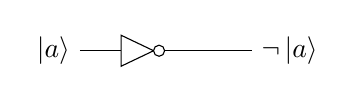
\begin{tikzpicture}
        \node[not gate US, draw, logic gate inputs=n] (neg) at (0,0){};
        \node (a) at (-1,0) {\(\ket{a}\)};
        \node (out) at (2,0) {\(\lnot \ket{a}\)};
        \draw (a) to (neg.input);
        \draw (neg.output) to (out);
    \end{tikzpicture}.
\end{center}
Na levi strani pišemo vhode (v tem primeru \(\ket{a}\)), črte pa predstavljajo kompozicijo oziroma tok podatkov. Tukaj gre bit \(\ket{a}\) v vrata za negacijo. Na desni strani vrat pa dobimo negiran bit. Takemu diagramu lahko rečemo vezje, ogledamo si še malo bolj zapleten primer. Tukaj predstavimo De Morganov zakon
\[
    \lnot(\ket{a}\land \ket{b}) = \lnot\ket{a} \lor \lnot \ket{b}
\]
\begin{center}
    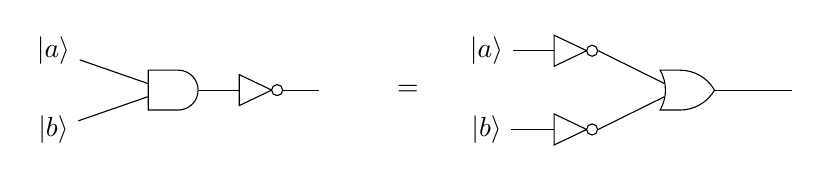
\begin{tikzpicture}
        \node[and gate US, draw, logic gate inputs=nn] (and) at (0,0){};
        \node[not gate US, draw, logic gate inputs=n] (neg) at (1,0){};
        \node (equal) at (3,0) {\(=\)};
        \node[or gate US, draw, logic gate inputs=nn] (or) at ($(equal)+(3.5,0)$){};
        \node[not gate US, draw, logic gate inputs=n] (nega) at ($(equal)+(2,0.5)$){};
        \node[not gate US, draw, logic gate inputs=n] (negb) at ($(equal)+(2,-0.5)$){};
        \node (a) at ($(equal)+(1,0.5)$) {\(\ket{a}\)};
        \node (b) at ($(equal)+(1,-0.5)$) {\(\ket{b}\)};
        \node (out) at ($(equal)+(5,0)$) {};
        \node (a1) at (-1.5,-0.5) {\(\ket{b}\)};
        \node (b1) at (-1.5,0.5) {\(\ket{a}\)};
        \node (out1) at (2,0) {};
        \draw (a1) to (and.input 2);
        \draw (b1) to (and.input 1);
        \draw (and.output) to (neg.input);
        \draw (neg.output) to (out1);
        \draw (a) to (nega.input);
        \draw (b) to (negb.input);
        \draw (or.output) to (out);
        \draw (nega.output) to (or.input 1);
        \draw (negb.output) to (or.input 2);
    \end{tikzpicture}.
\end{center}
Na levi strani imamo logična vrata za konjunkcijo, v katero vodita dva vhoda. Rezultat te operacije pa kasneje negiramo. Izhodne vrednosti dostikrat ne pišemo, saj bi bila enaka grafični predstavitvi vezja. Na desni strani enakosti pa vhode najprej negiramo, od tja pa podatke preusmerimo v vrata za disjunkcijo, iz katerih dobimo rezultat vezja. Po De Morganovem izreku sta vezji enaki.

Nazadnje si ogledamo še vrata \textsf{NAND}
\begin{center}
    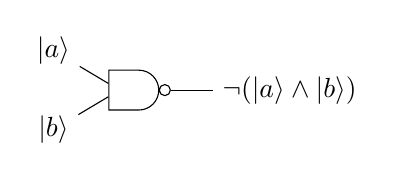
\begin{tikzpicture}
        \node[nand gate US, draw, logic gate inputs=nn] (nand) at (0,0){};
        \node (ina) at (-1, 0.5) {\(\ket{a}\)};
        \node (inb) at (-1, -0.5) {\(\ket{b}\)};
        \node (out) at (2, 0) {\(\lnot(\ket a\land \ket b)\)};
        \draw (ina) to (nand.input 1);
        \draw (inb) to (nand.input 2);
        \draw (nand.output) to (out);
    \end{tikzpicture},
\end{center}
vrata za negacijo z uporabo \textsf{NAND} pa bi bile
\begin{center}
    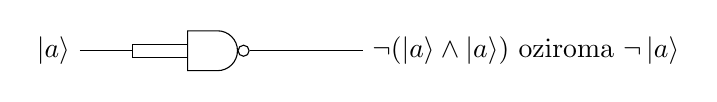
\begin{tikzpicture}
        \node[nand gate US, draw, logic gate inputs=nn] (nand) at (0,0){};
        \node (ina) at (-2, 0) {\(\ket{a}\)};
        \node (brunch) at (-1,0) {};
        \node (out) at (4, 0) {\(\lnot(\ket a\land \ket a)\) oziroma \(\lnot \ket{a}\)};
        \draw (ina) -- (-1,0) |- (nand.input 1);
        \draw (ina) -- (-1,0) |- (nand.input 2);
        \draw (nand.output) to (out);
    \end{tikzpicture}.
\end{center}
S pomočjo vrat za negacijo lahko enostavno izrazimo vrata za konjunkcijo, z De Morganovim zakonom pa tudi za disjunkcijo. Tako kmalu vidimo, da lahko poljubno vezje predstavimo le z vrati \textsf{NAND}.

\subsection{Implementacija}
Glavni razlog za grafični zapis vezij je podobnost z dejansko implementacijo v elektronskih vezjih. Logična vrata so enostavno dostopna, ponavadi implementirana s tranzistorji, povezave med njimi pa predstavljajo žice. Logične vrednosti predstavimo z električno napetostjo. Tako lahko za logično vrednost \(\ket1\) uporabimo \(+5\) V (pogosta je tudi vrednost \(+3.3\) V), za \(\ket0\) pa uporabimo \(0\) V.

%----------------------------------------------------------- KONEC KLASIČNO ------------------------------------------------------------------------------

\section{Kvantna mehanika}
Klasični pristop h kvantni mehaniki uporablja Hilbertove prostore \cite[stran 12]{mathforqm}.

\begin{definicija} \emph{Hilbertov prostor} \(\Hb\) je vektorski prostor s skalarnim produktom
    \begin{align*}
        \braket{\cdot}{\cdot} :& \Hb \times \Hb \to \C\\
        & (\psi, \varphi) \mapsto \braket{\psi}{\phi},
    \end{align*}
    za katerega za vse \(\phi, \psi, \varphi_1, \varphi_2 \in \Hb\) velja
    \begin{align*}
        \braket{\psi}{\varphi} &= \overline{\braket{\varphi}{\psi}},\\
        \braket\psi &\geq 0,\\
        \braket\psi = 0 &\iff \psi = 0,\\
        \forall a,b\in\C\sep \braket{\psi}{a\varphi_1 + b\varphi_2} &=a\braket{\psi}{\varphi_1} + b\braket{\psi}{\varphi_2}.
    \end{align*}
    Ta skalarni produkt pa inducira normo
    \begin{align*}
        \norm*{\cdot} : \Hb &\to \R\\
        \psi &\mapsto \sqrt{\braket\psi},
    \end{align*}
    v katerem je \(\Hb\) poln.
\end{definicija}

Linearnim preslikavam \(\Hb\to\Hb\) pravimo \emph{operatorji}. Če za operator \(A\) velja \(\forall \psi,\phi\in\Hb\sep\braket{A\psi}{\varphi} = \braket{\psi}{A\varphi}\), je \(A\) \emph{sebi-adjungirani operator}. Operator \(U\) je \emph{unitaren}, če velja \(\forall \psi,\varphi\in\Hb\sep \braket{U\psi}{U\varphi} = \braket{\psi}{\varphi}\).

Vektorje bomo pisali v Diracovem zapisu. Elementi \(\Hb\) so tako \(\ket{\psi}\in\Hb\), temu rečemo \emph{ket}. Znotraj skalarnih produktov ketov ponavadi ne pišemo, tako dobimo \(\braket{\ket\psi}{\ket\varphi} = \braket{\psi}{\varphi}\). Elementi dualnega prostora pa so \emph{braji}:
\begin{align*}
    \bra{\psi} \defeq \left(\varphi \mapsto \braket{\psi}{\varphi} \right).
\end{align*}
Tukaj opazimo, da velja \(\bra{\psi}\, \ket{\varphi} = \braket{\psi}{\varphi}\).

Pomembni so še lastni vektorji in projekcije: \(\ket{\psi}\) je \emph{lastni vektor} za \(A\) z \emph{lastno vrednostjo} \(\lambda\), če \(A\ket\psi = \lambda \ket\psi\); \(P\) je \emph{projekcija}, če \(P^2 = P\). Če je poleg tega \(P\) tudi sebi-adjungiran, je to \emph{ortogonalna projekcija}.

Za sestavljanje novih Hilbertovih prostorov iz starih nam bo služil tenzorski produkt. Ta nam bo omogočil, da združimo opis dveh kvantnih delcev v en sam sistem. Najprej definiramo \emph{tenzorski produkt} kot preslikavo
\begin{align*}
    \ket\varphi \otimes \ket\psi : \Hb_1 \times \Hb_2 &\to \mathbb C\\
    (u,v) &\mapsto \braket{u}{\varphi} \braket{v}{\psi}.
\end{align*}
Linearna ogrinjača takih vektorjev sestavi vektorski prostor \(\Hb_1 \otimes \Hb_2\). Če pišemo po komponentah in \(\ket\varphi\in\C^n\) ter \(\ket\psi\in\C^m\), potem bo tenzorski produkt teh dveh prostorov izomorfen \(\C^{nm}\), \(\ket\varphi\otimes\ket\psi\) pa bo ustrezal vektor, ki ima prvih \(n\) komponent enakih kot \(\ket\psi\) pomnožen s prvo komponento \(\ket\varphi\), naslednjih \(n\) komponent \(\ket\psi\) pomnožen z drugo komponento \(\ket\varphi\) in tako naprej. Podobno velja tudi v prostoru preslikav, kjer dobimo bločno matriko zmnoženih dimenzij.
\begin{align*}
    A\in \C^{n\times n}, B&\in\C^{m\times m}\\
    A\otimes B = \begin{bmatrix}
        a_{11}B&\cdots&a_{1n}B\\
        \vdots&\ddots&\vdots\\
        a_{n1}B&\cdots&a_{nn}B
    \end{bmatrix}&\in \C^{(nm)\times (nm)}
\end{align*}
Tenzorski produkt večih prostorov naredimo induktivno, najprej tenzorski produkt prvih dveh, dobljenega tenzorsko množimo s tretjim in tako naprej. Prav tako za elemente. Za to nam bo prav prišla oznaka
\begin{align*}
    \ket{\varphi}^{\otimes n} = \bigotimes_{j=1}^n \ket\varphi.
\end{align*}

\subsection{Von Neumannova slika}
\subsubsection{Spin}
\emph{Spin} je lastnost osnovnih delcov, podobno kot recimo njihova masa. Fizikalno je spin navidezno vrtenje delcev: imajo vrtilno količino, ampak se ne vrtijo. Za osnovne delce bi bilo dejansko vrtenje celo nesmiselno, saj so delci točkasti brez volumna ali polmera. Ne glede na to pa spin še vedno lahko izmerimo, prav tako pa ima mnoge posledice na okolje. V kvantnem računalništvu lahko spin uporabljamo za predstavitev kubitov -- analogije bitov v kvantnem računalništvu. 

\subsubsection{Kvantna stanja in opazljivke}
\emph{Kvantna stanja} so elementi Hilbertovega prostora \(\ket\psi\in\Hb\), za katere velja \(\norm{\ket\psi} = 1\). Najbolj osnoven primer so elementi oblike 
\begin{align*}
    \begin{bmatrix}a\\b\end{bmatrix} \in \C^2
\end{align*}
kjer \(a^2 + b^2 = 1\). Takemu stanju rečemo \emph{kubit}, bolj podrobno pa si jih bomo ogledali kasneje. \emph{Opazljivka} je merljiva količina kvantnega sistema (na primer hitrost ali pozicija). Predstavimo jo s sebi-adjungiranim operatorjem \(\Hb\). Kot primer opazljivke podamo opazljivke spina.
\begin{definicija} \label{Pauli} \emph{Paulijeve matrike} so \(2\times 2\) unitarne kompleksne matrike:
    \begin{align*}
        X &= \sigma_x \defeq \begin{bmatrix}
            0&1\\
            1&0
        \end{bmatrix},\\
        Y &= \sigma_y \defeq \begin{bmatrix}
            0&-i\\
            i&0
        \end{bmatrix},\\
        Z &= \sigma_z \defeq \begin{bmatrix}
            1&0\\
            0&-1
        \end{bmatrix}.
    \end{align*}
\end{definicija}
Opazljivke spina dobimo, če Paulijeve matrike delimo z \(2\). Te imajo lastne vrednosti \(\pm \frac12\) in jih uporabimo za meritve v naravi. V navadi pa je, da faktorja \(\frac12\) ne pišemo in kot opazljivke uporabimo le \(\sigma_x = X\) in \(\sigma_z = Z\) \cite[Definicija 2.21]{mathforqm}.
\subsubsection{Meritve}
V kvantnih sistemih lahko izmerimo opazljivke. Možni rezultati meritev so točno lastne vrednosti operatorja, ki predstavlja opazljivko. Definiramo \(P_\psi(\lambda)\) kot verjetnost, da za sistem v stanju \(\ket\psi\) dobimo po meritvi opazljivke \(A\) lastno vrednost \(\lambda\). Izkaže se, da je ta verjetnost enaka 
\begin{align*}
    P_\psi(\lambda) = \norm{P_\lambda \ket\psi}^2,
\end{align*}
kjer je \(P_\lambda\) projekcija na lastni podprostor za lastno vrednost \(\lambda\) \cite[Poglavje 2.3.1]{mathforqm}.

Definiramo oznako
\begin{align*}
    \ev{A}_\psi = \braket{\psi}{A\psi},
\end{align*}
ki jo imenujemo \emph{pričakovana vrednost} opazljivke \(A\) v stanju \(\ket\psi\). Če so \(e_j\) lastni vektorji \(A\) in \(\lambda_j\) njihove lastne vrednosti, lahko pričakovano vrednost razpišemo po lastni bazi
\begin{align*}
    \ev{A}_\psi = \sum_j\lambda_j\lvert \braket{\psi}{e_j}\rvert^2.
\end{align*}

\begin{izrek}
    Če je sistem pripravljen v stanju \(\ket\psi \in \Hb\) potem je verjetnost, da izmerimo stanje \(\ket\varphi \in \Hb\) enaka \(\lvert \braket{\varphi}{\psi}\rvert^2\).
\end{izrek}
\begin{proof}
    Opazljivka za preverjanje, če je sistem v stanju \(\varphi\) je kar projekcija \(P_\varphi = \ket\varphi \bra\varphi\). Ima lastno vrednost \(\lambda=1\) za lastni vektor \(\ket\varphi\), torej je projekcija na lastni podprostor tudi \(P_\varphi\).
    \begin{align*}
        P_\psi (\lambda) &= P_\psi(1) =\norm{P_1\ket\psi}^2 = \norm{P_\varphi\ket\psi}^2\\
                        &= \norm{\ket\varphi\braket{\varphi}{\psi}}^2 = \lvert \braket{\varphi}{\psi}\rvert^2,
    \end{align*}
    saj \(\norm{\ket\varphi} = 1\).
\end{proof}

Če izmerimo stanje \(\ket\psi\) za opazljivko \(A\) ter izmerimo lastno vrednost \(\lambda\), potem se stanje \(\ket\psi\) po meritvi spremeni v
\begin{align*}
    \frac{P_\lambda \ket\psi}{\norm{P_\lambda\ket\psi}}.
\end{align*}
Ta pojav je znan kot kolaps valovne funkcije, saj se pogosto (zaradi zgodovinskih razlogov) stanju \(\psi\) pravi valovna funkcija. Tudi, če smo imeli prej stanje, ki je linearna kombinacija večih vektorjev iz različnih lastnih podprostorov se bo z meritvijo stanje spremenilo in ne bo več linearna kombinacija, pač pa samo element enega lastnega podprostora. V enostavnem primeru, ko vsak lastni podprostor napenja natanko en vektor, če izmerimo \(\ket\psi\), naš vektor postane \(\ket\psi\), čeprav je bil prej lahko linearna kombinacija večih vektorjev. Po prejšnjem izreku pa imamo višje možnosti izmeriti bližnje lastne podprostore, povprečje pripadajočih lastnih vrednosti pa je natanko pričakovana vrednost \(\ev{A}_\psi\).

Oglejmo si primer meritve spina. Če opravimo meritev glede na opazljivko \(X\) lahko izmerimo lastno vrednost \(1\), kateri pripada lastni vektor \((1,0)\), ali pa lastno vrednost \(-1\), kateri pripada lastni vektor \((0,1)\). Torej ko izmerimo spin delca, se ta po meritvi pretvori v pripadajoči lastni vektor. Recimo da izmerimo spin delca \((a,b)\). Verjetnost, da izmerimo \(1\) je \(a^2\). Če pa se zgodi, da dejansko izmerimo \(1\), pa vemo, da je po meritvi delec v stanju \((1,0)\). Če ga nato še enkrat izmerimo bomo z verjetnostjo \(1\) ponovno izmerili lastno vrednost \(1\).
\subsection{Kubiti}
\emph{Kubiti} so elementi Hilbertovega prostora \(\mathbb C^2\) dolžine \(1\). Kot njihove opazljivke uporabimo Paulijeve matrike. Če gledamo le spin v \(z\) smeri, uporabljamo opazljivko \(\sigma_z\), ki ima lastni vrednosti \(\{+1, -1\}\). Tem lastnim vrednostim ustrezata lastna vektorja \(\ket0\) in \(\ket1\), katera definiramo kot
\begin{align*}
    \ket0 \defeq \begin{bmatrix}
        1\\0
    \end{bmatrix}\\
    \ket1 \defeq \begin{bmatrix}
        0\\1
    \end{bmatrix}.
\end{align*}
Opazimo, da to sestavlja bazo vektorskega prostora. Kubit lahko tako napišemo kot linearno kombinacijo \(\ket0\) in \(\ket1\). Tukaj lahko vidimo vzporednico s klasičnim računalništvom: tam so bili biti le \(\ket0\) in \(\ket1\), tukaj pa tudi vse vrednosti vmes! Eksplicitno, poljubni kubit je oblike \(a\ket0+b\ket1\) kjer \(a^2+b^2=1\).

Definiramo si še \emph{Bellovi stanji}
\begin{align*}
    \ket{+} \defeq \frac{1}{\sqrt2} (\ket0+\ket1)\\
    \ket{-} \defeq \frac{1}{\sqrt2} (\ket0-\ket1).
\end{align*}
Ustrezata lastnima vektorjema opazljivke \(\sigma_x\), ki spremlja spin v \(x\) smeri. Spin glede na \(X\) je dualen spinu glede na \(Z\), kar ima posledico, da ima vsak izrek o \(Z\) spinu analogno trditev o \(X\) spinu, le vse \(\ket+\) zamenjamo s \(\ket0\) in obratno, prav tako pa zamenjamo \(\ket-\) s \(\ket1\).

Podobno kot pri klasičnem računalniku potrebujemo sisteme z večimi biti, pri kvantnih računalnikih potrebujemo sisteme večih kubitov. Fizično ga pogosto predstavimo kot računalnik z večimi elektroni, po enim za vsak kubit. Tukaj uporabimo tenzorski produkt. Sistem dveh kubitov bi tako označili \(\mathbb C^2 \otimes \mathbb C^2\). Vpeljemo si še krajšo oznako za elemente:
\begin{align*}
    \ket{ab} \defeq& \ket{a}\otimes\ket{b}\\
    \ket{abc} \defeq& \ket{a}\otimes\ket{b}\otimes\ket{c}\\
    &\vdots
\end{align*}
S to oznako lahko preprosto napišemo poljuben element \(\mathbb C^2 \otimes \mathbb C^2\) kot
\begin{align*}
    a\ket{00} + b\ket{01} + c\ket{10} + d\ket{11}.
\end{align*}
Hitro opazimo, da dimenzija vektorskega prostora narašča eksponentno. Sistem dveh kubitov je dimenzije \(2^2\), sistem treh je \(2^3\), sistem \(n\) kubitov pa \(2^n\). Ta lastnost kvantnim računalnikom omogoča procesiranje velike količine podatkov z zelo majhnim številom kubitov.
\subsection{Prepletenost}
Ključni pojav kvantne mehanike za kvantno računalništvo je \emph{prepletenost}. Ta omogoča, da se več procesov odvija hkrati na način, ki ni prisoten v klasični fiziki. Če imamo dva kvantna sistema \(\Hb_1\) in \(\Hb_2\) (na primer dva elektrona), potem skupni sistem, katerega del sta oba sistema, opisuje \(\Hb_1\otimes\Hb_2\). Ta prostor pa je običajno večji kot prostor, ki vsebuje elemente oblike \(\ket\varphi\otimes\ket\psi\), saj je le generiran s takimi elementi in so v splošnem elementi oblike \(\sum_{i=0}^n a_i\ket{\varphi_i}\otimes\ket{\psi_i}\) za \(\ket{\phi_i}\in\Hb_1\), \(\ket{\psi_i}\in \Hb_2\) in \(a_i\in \C\). Splošen element lahko napišemo tudi kot linearno kombinacijo baznih vektorjev; če so \(\ket{\phi_i}\in \Hb_1\) in \(\ket{\psi_i}\in\Hb_2\) bazni vektorji in \(a_{ij}\) skalarji, je splošen element oblike \(\sum_{i=0}^n\sum_{j=0}^m a_{ij}\ket{\phi_i}\otimes\ket{\psi_j}\). Kadar lahko elemente napišemo kot ločen tenzorski produkt \(\ket\varphi\otimes\ket\psi\), pomeni da elementa nista prepletena in sta med seboj neodvisna.
\begin{definicija}
    Če se stanja \(\ket\gamma\in \Hb_1\otimes\Hb_2\) ne da napisati kot \(\ket\varphi\otimes\ket\psi = \ket\gamma\) za \(\ket\varphi\in\Hb_1\) in \(\ket\psi\in\Hb_2\), potem je \(\ket\gamma\) \emph{prepleteno kvantno stanje}.
\end{definicija}
Tako stanje
\begin{align*}
    \ket\psi &=  \frac12(\ket{00}+\ket{01}+\ket{10}+\ket{11})\\
    &= \frac{1}{\sqrt2}(\ket0+\ket1) \otimes \frac{1}{\sqrt2}(\ket0+\ket1) 
\end{align*}
ni prepleteno, ampak stanje \(\frac{1}{\sqrt2}(\ket{00}+\ket{11})\) pa je.
\subsection{Kvantna vrata} Pri klasičnih vratih so bila vrata na \(n\) bitov poljubne preslikave \(B^n\to B\). Kubiti pa pripadajo hilbertovemu prostoru, tako da se ustrezna analogija tukaj zdi \(\Hb^{\otimes n}\to \Hb\). Vemo pa, da morajo biti kvantni procesi brez meritev unitarne transformacije. To poskrbi, da se ohranjajo norme kvantnih stanj in da se, zaradi obrnljivosti, informacija ohranja. 
\begin{definicija}
    \emph{Kvantna vrata} na \(n\) kubitov so unitarni operatorji
    \begin{align*}
        U:\Hb^{\otimes n}\to \Hb^{\otimes n}.
    \end{align*}
    Če je \(n=1\) so to \emph{unarna kvantna vrata}, če je \(n=2\) pa \emph{binarna kvantna vrata} \cite[Definicija 5.7]{mathforqm}.
\end{definicija}
Ker so vrata predstavljena z unitarnimi preslikavami, jim torej ustrezajo tudi matrike. Te matrike navadno predstavimo v standardni bazi \(\ket0, \ket1\).

Najbolj enostaven primer kvantnih vrat je identiteta. To je preslikava, ki ji ustreza identična matrika (v standardni bazi). Omenili smo tudi Paulijeve matrike (definicija \ref{Pauli}), ki prav tako predstavljajo kvantna vrata. Tu že dobimo prvo preslikavo, ki je analogna pomembnim klasičnim vratom. Za Paulijevo \(X\) matriko velja \(X\ket0=\ket1\) in \(X\ket1=\ket0\), torej ustrezajo ravno negaciji. Pogosto jih imenujemo tudi \textsf{qNOT}, kar je okrajšava za ``\emph{quantum not}''. Pomembna so tudi Hadamardova vrata
\begin{align*}
    H &= \frac{1}{\sqrt{2}}(X+Z)\\
      &= \frac{1}{\sqrt2} \begin{bmatrix}
        1&1\\1&-1
    \end{bmatrix}.
\end{align*}
Ta ustrezajo menjavi baze, saj \(H\ket0=\ket+\) in \(H\ket1=\ket-\). 

Naslednja najenostavnejša vrata so vrata faznega faktorja
\begin{align*}
    M(\alpha) &= e^{i\alpha}\cdot \id\\
              &= \begin{bmatrix}
                  e^{i\alpha}&0\\
                  0&e^{i\alpha}
              \end{bmatrix}
\end{align*}
in sorodna vrata faznega zamika, ki so izjemno pomembna
\begin{align*}
    P(\alpha) &= \ket0\bra0 + e^{i\alpha}\ket1\bra1\\
              &= \begin{bmatrix}
                  1&0\\
                  0&e^{i\alpha}
              \end{bmatrix}.
\end{align*}
Eden izmed osnovnih elementov ZX-računa je v posebnem unarnem primeru namreč ravno \(P(\alpha)\). Najpogosteje so uporabljene faze \(\alpha=\frac\pi4\), kar imenujemo \(T\) vrata \(T=P(\frac\pi4)\) in pa \(\alpha=\frac\pi2\), kar imenujemo S vrata \(S = T^2=P(\frac\pi2)\).

Nazadnje omenimo še rotacijo okoli \(v=(v_x,v_y,v_z)\) za kot \(\alpha\)
\begin{align*}
    D_v(\alpha) = \begin{bmatrix}
        \cos\frac\alpha2 - iv_z\sin\frac\alpha2 & -i(v_x-iv_y)\sin\frac\alpha2\\
        -i(v_x+iv_y)\sin\frac\alpha2 & \cos\frac\alpha2 + v_zi\sin\frac\alpha2
    \end{bmatrix}.
\end{align*}
Zanimivo je, da lahko s slednjimi generiramo poljubno unitarno preslikavo na \(\Hb\) \cite[Lema 2.35]{mathforqm}. Kot primer velja 
\begin{align*}
    H = e^{i\frac{3\pi}{2}}D_z(0)D_y\left(\frac\pi2\right)D_z(-\pi),
\end{align*}
za \(y=(0,1,0)\) in \(z=(0,0,1)\).

Binarnim kvantnim vratom ustrezajo unitarne preslikave \(U:\Hb^{\otimes 2}\to \Hb^{\otimes 2}\), čemur ustrezajo \(4\times 4\) kompleksne matrike. Tu sta najbolj pomembni vrati \textsf{cNOT} 
\begin{align*}
    \mathsf{cNOT}&=\ket0\bra0\otimes I + \ket1\bra1\otimes X \\
    &=\begin{bmatrix}
        1&0&0&0\\
        0&1&0&0\\
        0&0&0&1\\
        0&0&1&0
    \end{bmatrix}
\end{align*}
in \textsf{swap}
\begin{align*}
    S &= \ket{00}\bra{00}+\ket{11}\bra{11}+\ket{01}\bra{10}+\ket{10}\bra{01}\\
    &=\begin{bmatrix}
        1&0&0&0\\
        0&0&1&0\\
        0&1&0&0\\
        0&0&0&1
    \end{bmatrix}.
\end{align*}
Vrata \textsf{swap} zamenjajo kubita \(S(x\otimes y)=y\otimes x\), \textsf{cNOT} pa prvega pustijo nespremenjenega, drugega pa negirajo \textsf{cNOT}\((x\otimes y)=x\otimes Xy\). Spet se lahko vprašamo, kako veliko množico kvantnih vrat potrebujemo, da predstavimo poljubna vrata.
\begin{definicija}
    Množica kvantnih vrat \(U=\{U_1,\ldots,U_j\}\) je \emph{univerzalna}, če lahko za poljubno število kubitov \(n\in\N\), poljubna vrata \(V:\Hb^n\to \Hb^n\) napišemo kot kombinacijo produktov vrat iz \(U\), tenzorskih produktov vrat iz \(U\) ter identitet poljubne velikosti.
\end{definicija}
Zgoraj omenjena vrata so že dovolj za univerzalnost, nabor pa bi lahko tudi zmanjšali. Dovolj je že družina \(\{D_x(\alpha),D_z(\alpha), M(\alpha), \mathsf{cNOT}\mid \alpha\in \R\}\) \cite[Lema 5.26]{mathforqm}.
\subsection{Kvantna vezja}
V veliki meri bi kvantna vezja lahko enačili s kvantnimi vrati. Vezja si namreč predstavljamo kot zaporedje vrat. Če pa vrata zmnožimo (tenzorsko za vzporedna vrata, navadno za zaporedna vrata) potem dobimo namreč novo unitarno preslikavo, kar so spet po definiciji kvantna vrata. Dodamo pa še nov element \emph{kvantne meritve}, ki pa ne ustreza kvantnim vratom, saj ni unitarna. Ta ustreza že prej omenjeni meritvi iz kvantne mehanike: kolapsira valovno funkcijo, izmeri lastno vrednost operatorja ter vrne projekcijo izmerjenega kubita na ustrezni lastni podprostor.

Unarna vrata predstavimo samo s črko ustreznega operatorja v kvadratu. Meritev opazljivke \(A\) predstavimo s simbolom
\begin{center}
    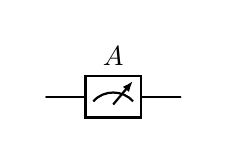
\begin{tikzpicture}
        \node {
            \begin{quantikz}
                \qw & \meter{A} & \qw
            \end{quantikz}  
        };
    \end{tikzpicture}
\end{center}
Če je \(A\) implicitno znana, je ne pišemo. 

Za binarne operatorje imamo posebne oznake. Vrata \textsf{cNOT} pišemo kot
\begin{center}
    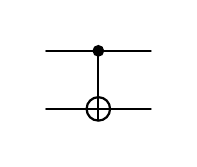
\begin{tikzpicture}
        \node {
            \begin{quantikz}
                \qw &  \ctrl{1} & \qw \\
                \qw &  \targ{}  & \qw
              \end{quantikz}
            };
    \end{tikzpicture},
\end{center}
vrata \textsf{swap} pa
\begin{center}
    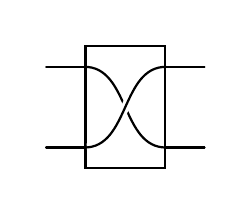
\begin{tikzpicture}
        \node {
            \begin{quantikz}
                \qw &  \gate[swap]{} & \qw \\
                \qw &  & \qw
              \end{quantikz}
            };
    \end{tikzpicture},
\end{center}
Za konec napišemo še primer malo večjega vezja. Tu na prvem kubitu izvedemo Hadamardova vrata, na drugem pa najprej vrata \(X\) ter nato Hadamardova. Nato na rezultatu obeh opravimo vrata \textsf{cNOT}.
\begin{center}
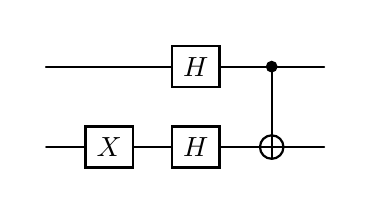
\begin{tikzpicture}
    \node[scale=1.0] {
      \begin{quantikz}
        \qw & \qw       & \gate{H} & \ctrl{1} & \qw \\
        \qw & \gate{X}  & \gate{H} & \targ{}  & \qw
      \end{quantikz}
    };
  \end{tikzpicture}
\end{center}

\subsection{Implementacija}
Za fizično implementacijo kvantnih vezij še ne poznamo najboljšega pristopa. Ne glede na pristop pa je pomembno, da lahko računalnik ustvari prepleteno stanje večih kubitov, ga obdrži za daljše obdobje nespremenjenega in na njem izvaja kvantna vrata (lahko se omejimo le na vrata iz univerzalnega nabora). Zaradi dekoherence pa je že to težavno, saj lahko tudi najmanjše zunanje motnje stanje spremenijo ali pa uničijo prepletenost. Da znižamo verjetnost, da se to zgodi imamo kvantni računalnik ohlajen na čim nižjo temperaturo, računalnik pa mora biti zaščiten od zunanjih tresljajev ali elektromagnetnih polij \cite[Poglavje 7.2]{nielsen}. 

Podajmo primer kvantnega računalnika preko harmoničnega oscilatorja. Harmonični oscilator je delec s potencialno energijo \(V(x)=m\omega^2x^2/2\), na primer masa na vzmeti ali pa električno vezje v resonanci, kjer energija oscilira med induktorjem in kondenzatorjem. Iz enačbe za potencialno energijo vidimo, da ima minimum v \(x=0\), okrog njega pa je simetrična. Na primeru vzmeti je \(x=0\) ravnovesna lega. Če vzmet potisnemo stran iz ravnovesne lege bo okoli nje oscilirala. Energija sistema se v tem primeru zvezno spreminja.

Zaradi kvantne narave pa je, če imamo sistem z zelo nizkim energijskim stanjem, energija diskretna funkcija, torej jemlje vrednosti iz diskretne množice števil. Energijska stanja lahko označimo \(\ket{n}\) kjer \(n\in \N\). Kubite lahko dobimo, če vzamemo končno podmnožico teh energijskih stanj \(\{\ket{ n } \mid 0\leq n \leq 2^k\}\) (predstavlja sistem \(k\) kubitov). Kvantna vrata predstavljajo, kako se sistem spreminja s časom. Izberemo le sistem, kjer se energija ustrezno spreminja ter izmerimo energijska stanja ob koncu transformacije. Slabost tega računalnika pa je, da je v celoti analogen ter zato težko izvedljiv v realnosti, ima pa lepe teoretične lastnosti. Tudi iskanje operatorja \(T\) pogosto ni enostavno \cite[Poglavje 7.3]{nielsen}.

Omenimo še nekaj ostalih pristopov. Pri fotonskih kvantnih računalnikih kubite predstavimo s polarizacijo svetlobe ali frekvenco, vrata pa predstavljajo elementi, ki se obnašajo kot ogledala in delilci svetlobe. Težavno je simulirati interakcijo med različnimi fotoni, kar ponavadi rešijo s Kerrovim efektom, ki omogoča, da se odbojni indeks materiala spremeni, če skozi njega potuje svetloba. Najbolj popularen pristop, ki neposredno uporablja spin delcov, pa je računalnik na jedrsko magnetno resonanco, računalnik s kvantnimi pikami ali pa s superprevodniki ohlajenimi pod kritično temperaturo. Kubite tu predstavlja spin delcev \cite{adamowski}.

%----------------------------- ZX-CALC -------------------------------------------

\section{ZX-račun}
V ZX-računu vezja predstavljamo z diagramom. To ima mnogo prednosti, saj so pogosto diagrami bolj pregledni ter njihovo poenostavljanje bolj preprosto. Ključno je, da lahko definiramo diagrame, ki so ekvivalentni vezju (oziroma predstavljajo linearne preslikave), vezja pa ustrezajo kvantnim procesom. Potem si definiramo dovoljene transformacije diagramov, ki ohranjajo pripadajoče linearne preslikave, vendar so naravne ter enostavne za uporabo. Cilj pa je, da z diagrami popolnoma nadomestimo klasični pogled (s klasičnimi kvantnimi vezji in pa linearnimi preslikavami) ter, kjer je mogoče, opisujemo lastnosti le z uporabo ZX-diagramov.
\subsection{Pajki}
Vozlišča v diagramu se imenujejo \emph{pajki}. Poznamo dva primarna tipa pajkov, pajek Z (barvamo zeleno) in pajek X (barvamo rdeče). Pajku pripada \emph{faza}, realno število, ki ga pišemo na sredini pajka (na skici je to \(\alpha\in\R\)).
\begin{center}
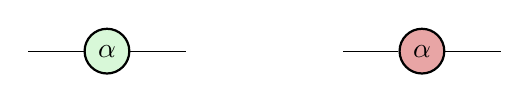
\begin{tikzpicture}
    \node [style=gn] (2) at (1,0) {\(\alpha\)};
    \node [style=rn] (1) at (5,0) {\(\alpha\)};
    \draw (0,0) to (2);
    \draw (2) to (2,0);
    \draw (4,0) to (1);
    \draw (1) to (6,0);
\end{tikzpicture}
\end{center}
Kadar je \(\alpha = 0\), faze ne pišemo, pajek ostane le zeleno ali rdeče pobarvan disk.

Lahko imata poljubno število vhodov ali izhodov. V temu članku bomo pisali vhode na levi strani, izhode pa na desni strani pajka (izkaže pa se, da to ne spremeni vezja, le pomaga intuiciji). Kot primer, Z pajek s tremi vhodi in dvema izhodoma je
\begin{center}
  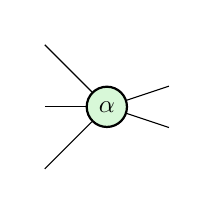
\begin{tikzpicture}[scale=0.9, every node/.style={scale=0.9}]
    \node (01) at (0, 0) {};
    \node (02) at (0, 1) {};
    \node (03) at (0, 2) {};
    \node [style=gn] (1) at (1.00, 1.00) {\(\alpha\)};
    \node (21) at (2, 0.66666) {};
    \node (22) at (2, 1.33333) {};
    \draw (01) to (1);
    \draw (02) to (1);
    \draw (03) to (1);
    \draw (1) to (21);
    \draw (1) to (22);
  \end{tikzpicture}.
\end{center}
Pajki ustrezajo linearnim preslikavam \cite[poglavje 1.1]{Backens}. Definiramo, da pajku Z z \(n\) vhodi in \(m\) izhodi pripada preslikava
\begin{align*}
    \ket{0}^{\otimes m} \bra{0}^{\otimes n} + e^{i\alpha}\ket{1}^{\otimes m} \bra{1}^{\otimes n}.
\end{align*}
To preslikavo lahko napišemo tudi kot \(2^n\times 2^m\) matriko. Element na mestu \((1,1)\) ustreza \(\ket{0}^{\otimes m} \bra{0}^{\otimes n}\) delu preslikave, element na mestu \((2^n, 2^m)\) pa \(\ket{1}^{\otimes m} \bra{1}^{\otimes n}\) delu preslikave. Če \((n,m)\neq (0,0)\) potem dobimo
\begin{align*}
    \begin{bmatrix}
        1 & 0 & \cdots & 0 \\
        0 & 0 & \cdots & 0 \\
        \vdots & \vdots & \ddots & 0 \\
        0 & 0 & 0 & e^{i\alpha} 
        \end{bmatrix}.
\end{align*}
Pajek brez vhodov ali izhodov s fazo \(\alpha\) pa napišemo kot skalar \(1+e^{i\alpha}\).
Podobno bi lahko definirali pajek X z \(n\) vhodi in \(m\) izhodi \cite[Poglavje 3.1]{workingcs} kot
\begin{align*}
    \ket{+}^{\otimes m} \bra{+}^{\otimes n} + e^{i\alpha}\ket{-}^{\otimes m} \bra{-}^{\otimes n}.
\end{align*}

To lahko posplošimo in definiramo operator \(\interpret{\cdot}: (D:n\to m)\to (\interpret{D}: \C^{2^n} \to \C^{2^m})\), ki poljubnemu diagramu (z \(n\) vhodi in \(m\) izhodi) priredi linearno preslikavo (\(2^n\times 2^m\) kompleksno matriko). V posebnem primeru \(n=m=0\) dobimo kompleksno število.

Da določimo matriko poljubnemu diagramu uporabljamo dve operaciji, \emph{tenzorski produkt} in pa \emph{kompozicijo} (oziroma navaden produkt). Z njima lahko kompleksne diagrame razbijemo na enostavne sestavne dele (posamezne pajke), katerim znamo dodeliti linearno preslikavo. Tenzorski produkt diagramov ustreza temu, da en diagram položimo nad drugega. Tako če imamo diagrama \(D\) in \(D'\) z \(n\) in \(n'\) vhodi ter \(m\) in \(m'\) izhodi, potem lahko naredimo diagram \(D\otimes D'\) z \(n+n'\) vhodi in \(m+m'\) izhodi. Analogno, kompozicija ustreza temu, da diagram položimo na desno (ter povežemo izhode desnega diagrama z vhodi levega). Tako če imamo diagram \(D:n\to m\) in diagram \(D':m\to k\), lahko definiramo diagram \(D'\circ D: n\to k\), kar ustreza temu, da \(D'\) položimo na desno od \(D\). Velja \(\interpret{D\otimes D'}\defeq \interpret{D} \otimes \interpret{D'}\), kar je tenzorski produkt pripadajočih matrik, in \(\interpret{D\circ D'} \defeq \interpret{D}\cdot \interpret{ D'}\), kar je produkt pripadajočih matrik. Kot primer, vzamemo dva enostavna diagrama \(D\) in \(D'\).
\begin{center}
    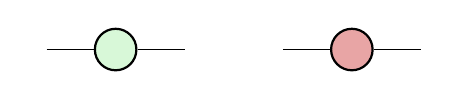
\begin{tikzpicture}
        \node (0) at (0,0) {};
        \node[style=gn] (1) at (1,0) {};
        \node (2) at (2,0) {};
        \node (3) at (3,0) {};
        \node[style=rn] (4) at (4,0) {};
        \node (5) at (5,0) {};
        \draw (1) to (2);
        \draw (0) to (1);
        \draw (3) to (4);
        \draw (4) to (5);
    \end{tikzpicture}
\end{center}
Njun tenzorski produkt je diagram \(D\otimes D':2\to 2\)
\begin{center}
    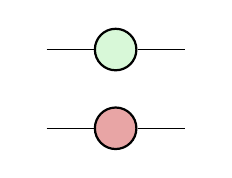
\begin{tikzpicture}
        \node (0) at (0,0) {};
        \node[style=rn] (1) at (1,0) {};
        \node (2) at (2,0) {};
        \node (3) at (0,1) {};
        \node[style=gn] (4) at (1,1) {};
        \node (5) at (2,1) {};
        \draw (1) to (2);
        \draw (0) to (1);
        \draw (3) to (4);
        \draw (4) to (5);
    \end{tikzpicture},
\end{center}
kompozicija pa \(D'\circ D: 1\to 1\)
\begin{center}
    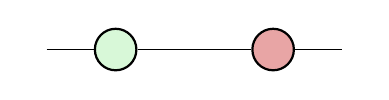
\begin{tikzpicture}
        \node (0) at (0,0) {};
        \node[style=gn] (1) at (1,0) {};
        \node[style=rn] (4) at (3,0) {};
        \node (5) at (4,0) {};
        \draw (1) to (4);
        \draw (0) to (1);
        \draw (4) to (5);
    \end{tikzpicture}.
\end{center}

\begin{definicija}
    Diagramu \(D:0\to0\) brez vhodov ali izhodov pravimo \emph{skalarni diagram}.
\end{definicija}
\begin{primer}\label{skal}
    Primer skalarnega diagrama, ki ga bomo pogosto uporabljali, je 
\begin{center}
    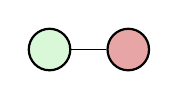
\begin{tikzpicture}
        \node[style=gn] (1) at (0,0) {};
        \node[style=rn] (2) at (1,0) {};
        \draw (1) to (2);
    \end{tikzpicture}.
\end{center}
Izračunamo, katero število mu ustreza.
\begin{align*}
    (\bra{+}+\bra{-})(\ket0 + \ket 1)&=
    \frac{1}{\sqrt2}(\bra{0}+\bra{1}+\bra0-\bra1)(\ket0 + \ket 1)\\
    &=\frac{2}{\sqrt2}(\braket{0}{0}+\braket{1}{0})\\
    &=\sqrt{2}\cdot (1 + 0) = \sqrt2
\end{align*}
Tako vidimo, da je interpretacija diagrama število \(\sqrt{2}\).
\end{primer}

Z uporabo pajkov in njihovih produktov si lahko definiramo nove konstrukcije. Tako lahko definiramo \emph{Hadamardova vrata} kot
\begin{center}
    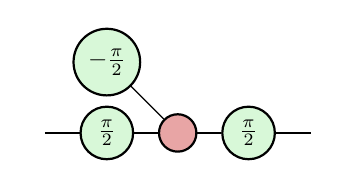
\begin{tikzpicture}[scale=0.9, every node/.style={scale=0.9}]
    \node (0) at (0.00, 0.00) {};
    \node [style=gn] (1) at (1, 0) {\(\frac\pi2\)};
    \node [style=gn] (a) at (1,1) {\(-\frac\pi2\)};
    \node [style=rn] (2) at (2, 0) {};
    \node [style=gn] (3) at (3, 0) {\(\frac\pi2\)};
    \node (4) at (4.00, 0.00) {};
    \draw (0) to (1);
    \draw (1) to (2);
    \draw (2) to (3);
    \draw (2) to (a);
    \draw (3) to (4);
    \end{tikzpicture}.
\end{center}
Ker jih bomo pogosto potrebovali, vpeljemo za ta vrata novo oznako
\begin{center}
    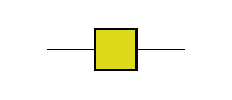
\begin{tikzpicture}
        \node (0) at (0, 0) {};
        \node [style=had] (h) at (1,0) {};
        \node (1) at (2,0) {};
        \draw (0) to (h);
        \draw (h) to (1);
    \end{tikzpicture}.
\end{center}
Kasneje bomo videli, da je, z uporabo teh vrat, diagram
\begin{center}
    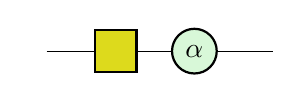
\begin{tikzpicture}
        \node (0) at (0, 0) {};
        \node [style=had] (h) at (1,0) {};
        \node [style=gn] (g) at (2,0) {\(\alpha\)};
        \draw (0) to (h);
        \draw (h) to (g);
        \draw (g) to (3,0);
    \end{tikzpicture}
\end{center}
ekvivalenten diagramu
\begin{center}
    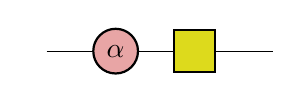
\begin{tikzpicture}
        \node (0) at (0, 0) {};
        \node [style=had] (h) at (2,0) {};
        \node [style=rn] (g) at (1,0) {\(\alpha\)};
        \draw (0) to (g);
        \draw (h) to (g);
        \draw (h) to (3,0);
    \end{tikzpicture}.
\end{center}
Ta lastnost je dejansko ključna za definicijo Hadamardovih vrat ter tudi pokaže zakaj so Hadamardova vrata pomembna, saj nam omogočajo menjavo baze (iz Z na X ali obratno). Lahko si tudi ogledamo matriko preslikave. To izračunamo tako, da vezje iz definicije razdelimo na manjše podenote. Matriko prvih dveh pajkov izračunamo kot tenzorski produkt matrik za oba posemezna pajka. Matriki za preostala pajka pa sledite po definiciji. Ostane le še, da združimo podenote, čemur ustreza matrično množenje.
\begin{align*}
    \begin{bmatrix}
        1&0\\0&i
    \end{bmatrix}\cdot \left(\ket{+}\bra{++}+\ket{-}\bra{--}\right)\cdot \left(\begin{bmatrix}
        1\\-i
    \end{bmatrix}\otimes\begin{bmatrix}
        1&0\\0&i
    \end{bmatrix}\right) =\\
    =\begin{bmatrix}
        1&0\\0&i
    \end{bmatrix}\cdot\left( \frac{1}{\sqrt2}\begin{bmatrix}
        1&0&0&1\\
        0&1&1&0
    \end{bmatrix}\right) \cdot
    \left(\begin{bmatrix}
        1 &0\\
        0 &i\\
        -i&0\\
        0 &1
    \end{bmatrix}
    \right)
\end{align*}
Tako Hadamardovim vratom ustreza matrika
\begin{align*}
    \frac{1}{\sqrt2}\begin{bmatrix}
        1&1\\
        1&-1
    \end{bmatrix},
\end{align*}
kar je ravno matrika, s katero smo definirali Hadamardova vrata s klasičnim pristopom. Enako bi dobili, če bi uporabili diagram 
\begin{center}
    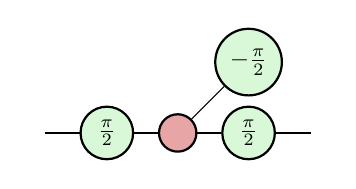
\begin{tikzpicture}[scale=0.9, every node/.style={scale=0.9}]
    \node (0) at (0.00, 0.00) {};
    \node [style=gn] (1) at (1, 0) {\(\frac\pi2\)};
    \node [style=gn] (a) at (3,1) {\(-\frac\pi2\)};
    \node [style=rn] (2) at (2, 0) {};
    \node [style=gn] (3) at (3, 0) {\(\frac\pi2\)};
    \node (4) at (4.00, 0.00) {};
    \draw (0) to (1);
    \draw (1) to (2);
    \draw (2) to (3);
    \draw (2) to (a);
    \draw (3) to (4);
    \end{tikzpicture},
\end{center}
kateremu ustreza linearna preslikava 
\begin{align*}
    \left(\begin{bmatrix}
        1&-i
    \end{bmatrix}\otimes\begin{bmatrix}
        1&0\\0&i
    \end{bmatrix}\right)\cdot \left(\frac{1}{\sqrt2}\begin{bmatrix}
        1&0\\
        0&1\\
        0&1\\
        1&0
    \end{bmatrix}\right) \cdot \begin{bmatrix}
        1&0\\0&i
    \end{bmatrix}.
\end{align*}
To dejstvo velja tudi za poljubne diagrame, zato jih lahko poljubno preoblikujemo, dokler ohranjamo povezave.

Tako smo definirali osnovne sestavne elemente ZX-diagramov. Brez operacij nad njimi pa so ti diagrami le navadni grafi, nepovezani s kvantno mehaniko ali kvantnimi procesi. Dovoljene operacije podamo kot seznam aksiomov, ki pripadajo ZX-računu.
\subsection{Aksiomi}
Za začetek bomo uporabili aksiomatizacijo za splošen ZX-račun podano v \cite[poglavje 2.2]{vilmart}, obstajajo pa tudi nekatere razširitve in različice, prav tako pa alternativne izbire aksiomov.

Aksiomi ZX-diagramov so zelo simetrični. Če neka lastnost velja za diagrame z zelenimi pajki Z, velja tudi, če te pajke spremenimo v rdeče pajke X. Tudi bolj splošno velja: za vsak aksiom obstaja dualni aksiom, kjer so povezave in faze identične, barve pa zamenjamo. Torej lahko zamenjamo tudi barvo pravil, ki vsebujejo mešane pajke (in ne le samo enobarvnih). Dodatno, vsi predstavljeni aksiomi so ekvivalence, torej za njih držijo lastnosti ekvivalenčnih relacij. Posebej je treba poudariti simetričnost: pravila delujejo tudi v obratno smer. Ko aksiom pravi, da lahko sosednje pajke združimo bi prav tako lahko samotarskega pajka ločili v več novih (dokler ga lahko z enakim aksiomom združimo nazaj v prvotnega).

Aksiome se ponavadi uporablja kot pravila prepisovanja, podobno kot pri poenostavljanju enačb (le da tukaj poenostavljamo vezja). Tako kot lahko pri enačbah vedno \(1\) zamenjamo z \(\cos(0)\), ne glede na to kje v izrazu se nahaja, lahko tu podgraf zamenjamo z ekvivalentnim podgrafom.

\subsubsection{Topologija} Prvi in ključni aksiom ZX-diagramov je, da lahko povezave med pajki poljubno ukrivimo, s tem pa ne spremenimo pomena vezja.
Tako, na primer
\begin{center}
    \begin{tikzpicture}[scale=0.9, every node/.style={scale=0.9}]
                \node [style=none] (0) at (-4, 0) {};
                \node [style=none] (1) at (-2, -1) {};
                \node [style=none] (2) at (-2, 0) {};
                \node [style=none] (3) at (-2, 1) {};
                \node [style=none] (4) at (0, 0) {};
                \node [style=none] (5) at (0.75, 0) {\(=\)};
                \node [style=none] (6) at (4.25, 0) {\(=\)};
                \node [style=none] (7) at (5, 0) {};
                \node [style=none] (8) at (7, 1) {};
                \node [style=none] (9) at (7, 0) {};
                \node [style=none] (10) at (7, -1) {};
                \node [style=none] (11) at (9, 0) {};
                \node [style=none] (12) at (1.5, 0) {};
                \node [style=none] (13) at (3.5, 0) {};
                \draw [in=180, out=0] (0.center) to (1.center);
                \draw [bend right=90, looseness=2.25] (1.center) to (2.center);
                \draw [bend right=270, looseness=2.00] (2.center) to (3.center);
                \draw [in=180, out=0] (3.center) to (4.center);
                \draw (12.center) to (13.center);
                \draw [in=-180, out=0] (7.center) to (8.center);
                \draw [bend left=90, looseness=2.25] (8.center) to (9.center);
                \draw [bend right=90, looseness=2.00] (9.center) to (10.center);
                \draw [in=-180, out=0] (10.center) to (11.center);
    \end{tikzpicture}.
\end{center}
Podobno lahko razrešimo vozle
\begin{center}
    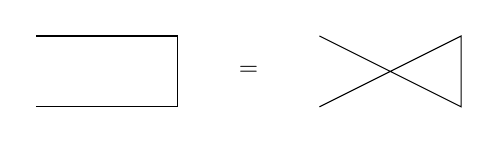
\begin{tikzpicture}[scale=0.9, every node/.style={scale=0.9}]
        \node (0) at  (0,0) {};
        \node (1) at (2,0) {};
        \node (2) at (2,1) {};
        \node (3) at (0,1) {};
        \node (eq) at (3,0.5) {=};
        \node (0a) at (4,0) {};
        \node (1a) at (6,0) {};
        \node (2a) at (6,1) {};
        \node (3a) at (4,1) {};
        \draw (0.center) -- (1.center) -- (2.center) to (3.center);
        \draw (0a.center) -- (2a.center) -- (1a.center) to (3a.center);
    \end{tikzpicture}.
\end{center}

Zanimivo in pomembno je tudi, da se topološka ekvivalenca prenese na vhode in izhode vrat.
\begin{center}
    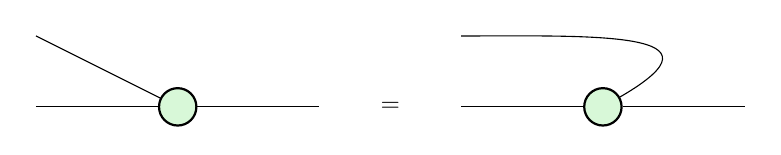
\begin{tikzpicture}[scale=0.9, every node/.style={scale=0.9}]
        \node (0) at (0, 1) {};
		\node (1) at (0, 0) {};
		\node[style=gn] (2) at (2, 0) {};
		\node (3) at (4, 0) {};
		\node (4) at (6, 0) {};
		\node[style=gn] (5) at (8, 0) {};
        \node (eq) at (5,0) {\(=\)};
		\node (6) at (10, 0) {};
		\node (7) at (6, 1) {};
        \draw (1.center) to (2);
		\draw (0.center) to (2);
		\draw (2) to (3.center);
		\draw (4.center) to (5);
		\draw (5) to (6.center);
		\draw [in=30, out=0, looseness=2.00] (7.center) to (5);
    \end{tikzpicture}
\end{center}
Torej je težko govoriti o vhodih ali izhodih pajkov, saj lahko vsak vhod spremenimo v izhod (in s tem ne spremenimo vezja) in tudi obratno. Še vedno pa nam to pomaga pri intuiciji in opisu diagramov, tako da povezavam, ki prihajajo iz leve strani, pravimo vhodi, tistim na desni strani pajka pa izhodi. Pogosto pa zaradi lepšega izgleda povezavo pustimo kar navpično. Prej smo ekvivalenco topološko preurejenih diagramov že preverili na primeru Hadamardovih vrat. Podobno bi lahko preverili tudi za ostale diagrame, na primer vrata \textsf{cNOT}. 
\begin{center}
    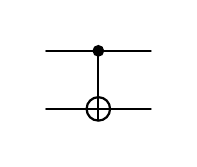
\begin{tikzpicture}
        \node (quantum) at (0,0.5) {
          \begin{quantikz}
            \qw & \ctrl{1} & \qw \\
            \qw & \targ{}  & \qw
          \end{quantikz}
        };
        \end{tikzpicture}
\end{center}
V ZX lahko ta vrata napišemo kot katerikoli izmed slednjih diagramov.
\begin{center}
    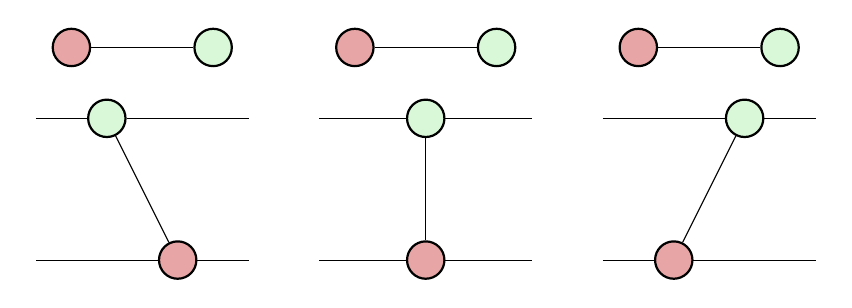
\begin{tikzpicture}[scale=0.9, every node/.style={scale=0.9}]
            \node [style=rn] (1r) at (-5.5, 2) {};
            \node [style=gn] (1g) at (-3.5,2) {};
            \node [style=rn] (2r) at (-1.5, 2) {};
            \node [style=gn] (2g) at (0.5,2) {};
            \node [style=rn] (3r) at (2.5, 2) {};
            \node [style=gn] (3g) at (4.5,2) {};
            \node [style=none] (2) at (-2, 1) {};
            \node [style=none] (3) at (-2, -1) {};
            \node [style=none] (4) at (1, 1) {};
            \node [style=none] (5) at (1, -1) {};
            \node [style=none] (6) at (2, 1) {};
            \node [style=none] (7) at (2, -1) {};
            \node [style=none] (8) at (-3, 1) {};
            \node [style=none] (9) at (-3, -1) {};
            \node [style=none] (10) at (-6, -1) {};
            \node [style=none] (11) at (-6, 1) {};
            \node [style=none] (12) at (5, 1) {};
            \node [style=none] (13) at (5, -1) {};
            \node [style=gn] (14) at (-5, 1) {}; %levo
            \node [style=gn] (15) at (4, 1) {}; % desno
            \node [style=gn] (16) at (-0.5, 1) {}; % sredina
            \node [style=rn] (17) at (-4, -1) {};
            \node [style=rn] (18) at (-0.5, -1) {};
            \node [style=rn] (19) at (3, -1) {};
            \draw (11.center) to (14);
            \draw (14) to (8.center);
            \draw (14) to (17);
            \draw (17) to (9.center);
            \draw (17) to (10.center);
            \draw (2.center) to (16);
            \draw (16) to (4.center);
            \draw (16) to (18);
            \draw (3.center) to (18);
            \draw (18) to (5.center);
            \draw (6.center) to (15);
            \draw (15) to (12.center);
            \draw (15) to (19);
            \draw (7.center) to (19);
            \draw (19) to (13.center);
            \draw (1r) to (1g);
            \draw (2r) to (2g);
            \draw (3r) to (3g);
    \end{tikzpicture}    
\end{center}
Opazimo, da smo lahko pajka premaknili tudi naprej ali nazaj. Dovoljeno je poljubno premikanje pajkov po ravnini, dokler ne spremenimo, kako so povezani.

Ta pravila skupaj nam upravičijo uporabo matematičnih grafov, kot poznanih iz teorije grafov. Tam lahko prav tako vozlišča premikamo po ravnini, povezave lahko ukrivljamo, prav tako pa ni pomembno v katero stran vozlišča vodi povezava, dokler je le pripeta. Pogosto je uporabljen slogan ``\emph{only connectivity matters}'' -- glede oblike so pomembne samo povezave.

Treba pa je poudariti, da v ostalih aksiomih prostega konca vhodnih in izhodnih povezav ne smemo premikati. Razlog je ravno v tem, da aksiome uporabljamo kot pravila prepisovanja; prosti konec povezave je le ena polovica povezave, ki je vidna v našem poddiagramu (druga polovica pa se nahaja v diagramu, ki ga poenostavljamo). Če bi premikali tudi prosti konec, bi lahko močno spremenili pomen. Poglejmo si na primeru, kjer smo ohranili vse povezave, premaknili smo le proste konce.
\begin{center}
    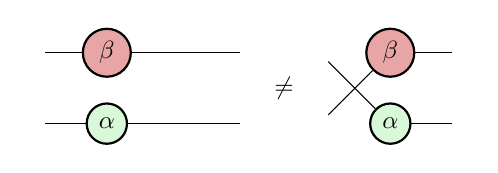
\begin{tikzpicture}[scale=0.9, every node/.style={scale=0.9}]
        \node (0) at (0,0) {};
        \node[style=gn] (1) at (1,0) {\(\alpha\)};
        \node[style=rn] (2) at (1,1) {\(\beta\)};
        \node (3) at (0,1) {};
        \node (0a) at (4,0) {};
        \node[style=gn] (1a) at (5,0) {\(\alpha\)};
        \node[style=rn] (2a) at (5,1) {\(\beta\)};
        \node (3a) at (4,1) {};
        \node (neq) at (3.5,0.5) {\(\neq\)};
        \node (end1) at (3,0) {};
        \node (end2) at (3,1) {};
        \node (end3) at (6,0) {};
        \node (end4) at (6,1) {};        
        \draw (0) to (1);
        \draw (2) to (3);
        \draw (0a) to (2a);
        \draw (1a) to (3a);
        \draw (1) to (end1);
        \draw (2) to (end2);
        \draw (1a) to (end3);
        \draw (2a) to (end4);
    \end{tikzpicture}
\end{center}
Če bi poskusili to pravilo uporabiti v diagramu 
\begin{center}
    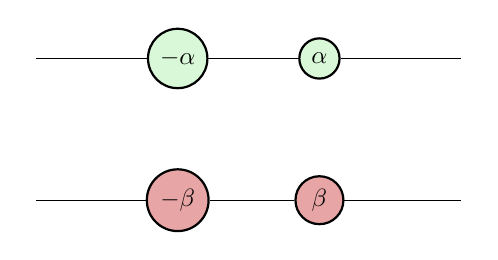
\begin{tikzpicture}[scale=0.9, every node/.style={scale=0.9}]
            \node [style=gn] (0) at (-1, 1) {\(-\alpha\)};
            \node [style=gn] (1) at (1, 1) {\(\alpha\)};
            \node [style=rn] (2) at (-1, -1) {\(-\beta\)};
            \node [style=rn] (3) at (1, -1) {\(\beta\)};
            \node [style=none] (4) at (-3, 1) {};
            \node [style=none] (5) at (-3, -1) {};
            \node [style=none] (6) at (3, 1) {};
            \node [style=none] (7) at (3, -1) {};
            \draw (4.center) to (0);
            \draw (0) to (1);
            \draw (6.center) to (1);
            \draw (3) to (7.center);
            \draw (3) to (2);
            \draw (2) to (5.center);
    \end{tikzpicture},
\end{center}
bi dobili
\begin{center}
    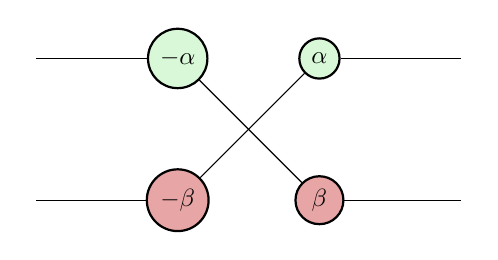
\begin{tikzpicture}[scale=0.9, every node/.style={scale=0.9}]
            \node [style=gn] (0) at (-1, 1) {\(-\alpha\)};
            \node [style=gn] (1) at (1, 1) {\(\alpha\)};
            \node [style=rn] (2) at (-1, -1) {\(-\beta\)};
            \node [style=rn] (3) at (1, -1) {\(\beta\)};
            \node [style=none] (4) at (-3, 1) {};
            \node [style=none] (5) at (-3, -1) {};
            \node [style=none] (6) at (3, 1) {};
            \node [style=none] (7) at (3, -1) {};
            \draw (4.center) to (0);
            \draw (6.center) to (1);
            \draw (3) to (7.center);
            \draw (2) to (5.center);
            \draw (0) to (3);
            \draw (1) to (2);
    \end{tikzpicture}
\end{center}
oziroma 
\begin{center}
    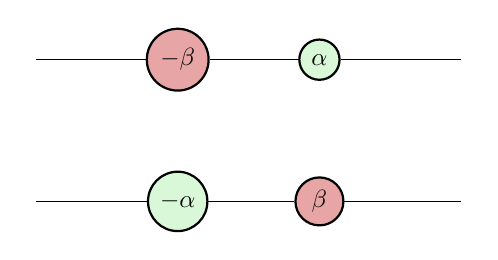
\begin{tikzpicture}[scale=0.9, every node/.style={scale=0.9}]
            \node [style=gn] (0) at (-1, -1) {\(-\alpha\)};
            \node [style=gn] (1) at (1, 1) {\(\alpha\)};
            \node [style=rn] (2) at (-1, 1) {\(-\beta\)};
            \node [style=rn] (3) at (1, -1) {\(\beta\)};
            \node [style=none] (4) at (-3, -1) {};
            \node [style=none] (5) at (-3, 1) {};
            \node [style=none] (6) at (3, 1) {};
            \node [style=none] (7) at (3, -1) {};
            \draw (4.center) to (0);
            \draw (6.center) to (1);
            \draw (3) to (7.center);
            \draw (2) to (5.center);
            \draw (0) to (3);
            \draw (1) to (2);
    \end{tikzpicture}.
\end{center}
Kar pa za večino faz ne bo ekvivalentno! Izvorni diagram namreč je ekvivalenten identiteti (za kar potrebujemo še nekaj dodatnih aksiomov), izpeljani pa za recimo \(\alpha = \beta = \frac\pi2\) ni.

Torej si predstavljamo, da so prosti konci togo vpeti v ravnino (ali pa vsaj ohranijo isto povezavo v naddiagramu, ko uporabimo pravilo).
% ----------------------------- aksiomi --------------------------------------------------------------------------------
\subsubsection{Identiteta} \label{identiteta}
Če imamo pajka s fazo \(0\) in z natanko enim vhodom in izhodom, je to vezje ekvivalentno identiteti
\begin{center}
    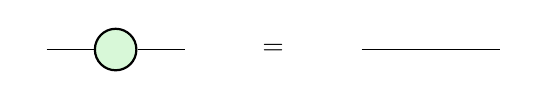
\begin{tikzpicture}
        \node (1) at (0,0) {};
        \node[style=gn] (gn) at (1,0) {};
        \node (2) at (2,0) {};
        \node (eq) at (3,0) {\(=\)};
        \node (4) at (4,0) {};
        \node (5) at (6,0) {};
        \draw (1) to (gn) to (2); 
        \draw (4) to (5);
    \end{tikzpicture}.
\end{center}
Skladnost aksiomov z Von Neumannovim pristopom lahko preverimo tako, da izračunamo pripadajočo matriko.
\begin{align*}
    \ket0\bra0 + \ket1\bra1 = \begin{bmatrix}
        1&0\\0&1
    \end{bmatrix}
\end{align*}
Enako bi lahko preverili matriko dualnega aksioma, ekvivalence rdečega pajka in identitete.
\begin{align*}
    (\ket+\bra+) +(\ket-\bra-)&=
    \frac{1}{2} ((\ket0+\ket1)(\bra0 + \bra1)) + \frac{1}{2}((\ket0-\ket1)(\bra0 - \bra1))\\
    &=\frac{1}{2} (2\ket0\bra0 + 2\ket0\bra1)\\
    &=\begin{bmatrix}
        1&0\\0&1
    \end{bmatrix}
\end{align*}
Podobno lahko za ostale aksiome naredimo enostaven račun, zato za njih skladnosti ne bomo preverjali.
\subsubsection{Združitev pajkov} \label{zdruzitev}
Sosednje pajke iste barve lahko združimo, dokler ohranimo isto število skupnih vhodov in izhodov. Pri tem se faze seštejejo.
\begin{center}
    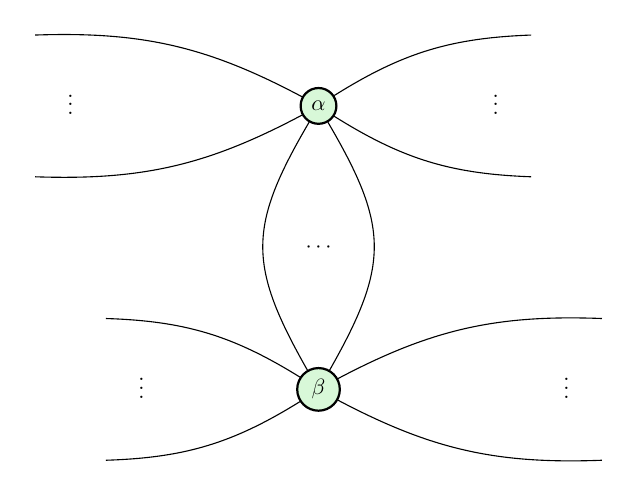
\begin{tikzpicture}[scale=0.9, every node/.style={scale=0.8}]
        \node [style=gn] (0) at (0, 2) {\(\alpha\)};
        \node [style=gn] (1) at (0, -2) {\(\beta\)};
        \node [style=none] (2) at (4, -1) {};
        \node [style=none] (3) at (4, -3) {};
        \node [style=none] (4) at (-4, 3) {};
        \node [style=none] (5) at (-4, 1) {};
        \node [style=none] (6) at (3, 3) {};
        \node [style=none] (7) at (3, 1) {};
        \node [style=none] (8) at (-3, -1) {};
        \node [style=none] (9) at (-3, -3) {};
        \node [style=none] (10) at (2.5, 2) {\(\rvdots\)};
        \node [style=none] (12) at (-2.5, -2) {\(\rvdots\)};
        \node [style=none] (13) at (3.5, -2) {\(\rvdots\)};
        \node [style=none] (14) at (0, 0) {\(\cdots\)};
        \node [style=none] (15) at (-3.5, 2) {\(\rvdots\)};
        \draw [bend left=15] (4.center) to (0);
        \draw [bend right=15] (5.center) to (0);
        \draw [bend right=15] (2.center) to (1);
        \draw [bend left=15] (3.center) to (1);
        \draw [bend right, looseness=1.25] (0) to (1);
        \draw [bend left, looseness=1.25] (0) to (1);
        \draw [bend left=15] (0) to (6.center);
        \draw [bend right=15] (0) to (7.center);
        \draw [bend left=15] (8.center) to (1);
        \draw [bend right=15] (9.center) to (1);
    \end{tikzpicture}
\end{center}
lahko prepišemo v
\begin{center}
    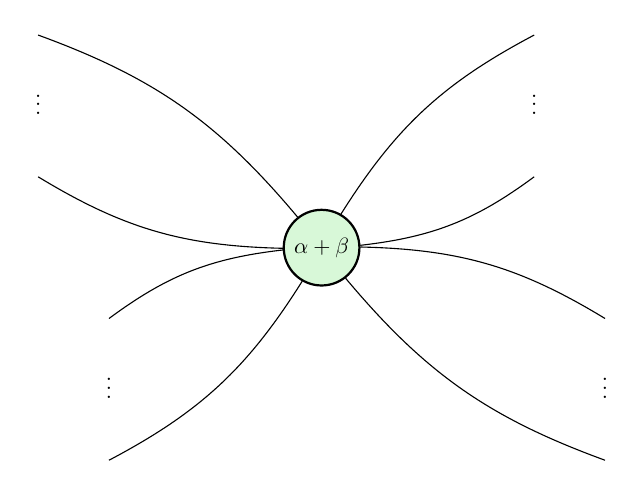
\begin{tikzpicture}[scale=0.9, every node/.style={scale=0.8}]
            \node [style=gn] (0) at (0, 0) {\(\alpha+\beta\)};
            \node [style=none] (1) at (-4, 3) {};
            \node [style=none] (2) at (-4, 1) {};
            \node [style=none] (3) at (-3, -1) {};
            \node [style=none] (4) at (-3, -3) {};
            \node [style=none] (5) at (4, -1) {};
            \node [style=none] (6) at (4, -3) {};
            \node [style=none] (7) at (3, 3) {};
            \node [style=none] (8) at (3, 1) {};
            \node [style=none] (9) at (-4, 2) {\(\rvdots\)};
            \node [style=none] (10) at (-3, -2) {\(\rvdots\)};
            \node [style=none] (11) at (3, 2) {\(\rvdots\)};
            \node [style=none] (12) at (4, -2) {\(\rvdots\)};
            \draw [bend left=15] (1.center) to (0);
            \draw [bend right=15] (2.center) to (0);
            \draw [bend left=15] (3.center) to (0);
            \draw [bend right=15] (4.center) to (0);
            \draw [bend right=15] (7.center) to (0);
            \draw [bend left=15] (8.center) to (0);
            \draw [bend right=15] (5.center) to (0);
            \draw [bend left=15] (6.center) to (0);
    \end{tikzpicture}.
\end{center}
Med pajkoma mora biti vsaj ena povezava, pravih vhodov ali izhodov pa je lahko tudi nič.

Aksioma za združitev pajkov in identiteto ustrezata aksiomatizaciji ortonormirane baze \cite[poglavje 5]{coecke_pavlovic_vicary_2013}.

\subsubsection{Izničenje pajkov} \label{iznicenje}
Povezani pajki določenih faz so ekvivalentni praznemu diagramu. Aksiom definira, da lahko diagrame oblike
\begin{center}
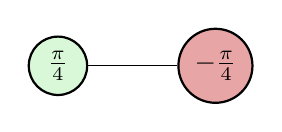
\begin{tikzpicture}
		\node [style=rn] (0) at (2, 0) {\(-\frac\pi4\)};
		\node [style=gn] (1) at (0,0) {\(\frac\pi4\)};
		\draw (0) to (1);
\end{tikzpicture}
\end{center}
preprosto izbrišemo. Prazen diagram ustreza skalarju \(1\), torej je ta diagram ekvivalenten skalarju \(1\). To je edini aksiom, ki nam lahko ustvari prazen diagram.
%
%Kot zanimivost, podvojeno različico tega pravila lahko izpeljemo tudi brez zgornjega pravila \cite[poglavje 3.1]{jeandel_et_al}! Tako je tudi
%\begin{center}
%    \begin{tikzpicture}[scale=0.9, every node/.style={scale=0.9}]
%            \node [style=rn] (0) at (2, 0) {\(-\frac\pi4\)};
%            \node [style=gn] (1) at (0, 0) {\(\frac\pi4\)};
%            \node [style=rn] (00) at (2, 1.5) {\(-\frac\pi4\)};
%            \node [style=gn] (11) at (0, 1.5) {\(\frac\pi4\)};
%            \draw (0) to (1);
%            \draw (00) to (11);
%    \end{tikzpicture}
%\end{center}
%ekvivalenten skalarju \(1\).
%
\subsubsection{Bialgebra} \label{bialgebra}
Pravilo bialgebre nam pove, kako lahko poenostavljamo diagrame, kjer so povezani pajki različnih barv.
\begin{center}
    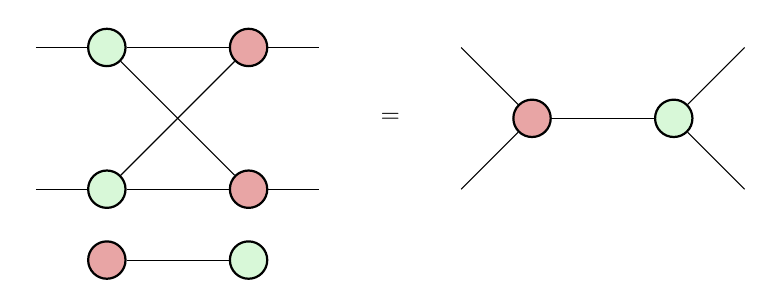
\begin{tikzpicture}[scale=0.9, every node/.style={scale=0.9}]
            \node [style=gn] (0) at (-3, 0) {};
            \node [style=gn] (1) at (-3, 2) {};
            \node [style=gn] (2) at (-1, -1) {};
            \node [style=rn] (3) at (-3, -1) {};
            \node [style=rn] (4) at (-1, 0) {};
            \node [style=rn] (5) at (-1, 2) {};
            \node [style=none] (6) at (-4, 0) {};
            \node [style=none] (7) at (-4, 2) {};
            \node [style=none] (8) at (0, 0) {};
            \node [style=none] (9) at (0, 2) {};
            \node [style=none] (10) at (1, 1) {\(=\)};
            \node [style=rn] (11) at (3, 1) {};
            \node [style=gn] (12) at (5, 1) {};
            \node [style=none] (13) at (2, 0) {};
            \node [style=none] (14) at (2, 2) {};
            \node [style=none] (15) at (6, 0) {};
            \node [style=none] (16) at (6, 2) {};
            \draw (6.center) to (0);
            \draw (7.center) to (1);
            \draw (0) to (4);
            \draw (4) to (8.center);
            \draw (1) to (5);
            \draw (5) to (9.center);
            \draw (3) to (2);
            \draw (0) to (5);
            \draw (1) to (4);
            \draw (11) to (12);
            \draw (12) to (15.center);
            \draw (12) to (16.center);
            \draw (11) to (14.center);
            \draw (11) to (13.center);
    \end{tikzpicture}    
\end{center}

\subsubsection{Pravilo kopiranja} \label{kopiranje}
Ta aksiom nam omogoča, da vhod ``kopiramo''. Izvorna informacija prihaja iz enega rdečega pajka, s tem pravilom pa je to ekvivalentno temu, da dva nepovezana pajka informacijo pošiljata naprej.
\begin{center}
    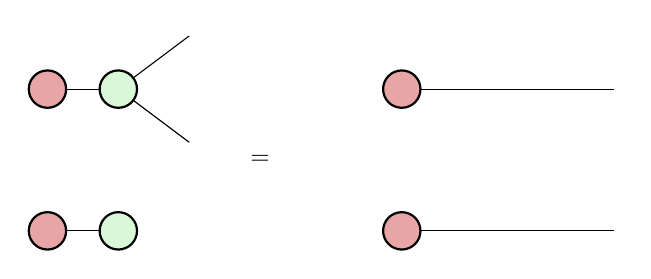
\begin{tikzpicture}[scale=0.9, every node/.style={scale=0.9}]
            \node [style=rn] (0) at (-3, -1) {};
            \node [style=rn] (1) at (-3, 1) {};
            \node [style=gn] (2) at (-2, -1) {};
            \node [style=gn] (3) at (-2, 1) {};
            \node [style=none] (4) at (-1, 0.25) {};
            \node [style=none] (5) at (-1, 1.75) {};
            \node [style=none] (7) at (0, 0) {\(=\)};
            \node [style=rn] (8) at (2, -1) {};
            \node [style=rn] (9) at (2, 1) {};
            \node [style=none] (10) at (5, -1) {};
            \node [style=none] (11) at (5, 1) {};
            \draw (0) to (2);
            \draw (1) to (3);
            \draw (3) to (4.center);
            \draw (3) to (5.center);
            \draw (8) to (10.center);
            \draw (9) to (11.center);
    \end{tikzpicture}      
\end{center}

\subsubsection{Hadamardova dekompozicija} \label{had-dekomp}
Lahko naredimo dekompozicijo Hadamardovih vrat z uporabo \(\frac\pi2\) rotacij.
\begin{center}
    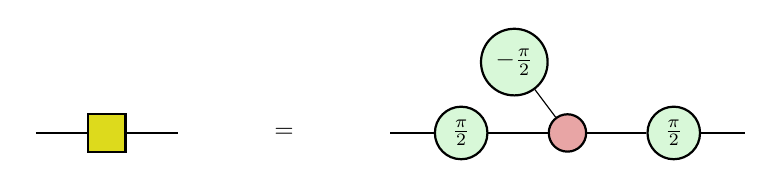
\begin{tikzpicture}[scale=0.9, every node/.style={scale=0.9}]
        \node [style=none] (0) at (-5, 0) {};
		\node [style=none] (1) at (-3, 0) {};
		\node [style=had] (2) at (-4, 0) {};
		\node [style=none] (4) at (-1.5, 0) {\(=\)};
		\node [style=none] (5) at (0, 0) {};
		\node [style=none] (6) at (5, 0) {};
		\node [style=rn] (7) at (2.5, 0) {};
		\node [style=gn] (8) at (1, 0) {\(\frac\pi2\)};
		\node [style=gn] (9) at (4, 0) {\(\frac\pi2\)};
		\node [style=gn] (10) at (1.75, 1) {\(-\frac\pi2\)};
		\draw (0.center) to (2);
		\draw (2) to (1.center);
		\draw (5.center) to (8);
		\draw (8) to (7);
		\draw (7) to (9);
		\draw (9) to (6.center);
		\draw (7) to (10);
    \end{tikzpicture}    
\end{center}

\subsubsection{Hadamardova menjava barv} \label{had-menjava}
Hadamardova vrata lahko uporabimo za menjavo barve pajka tako, da na vse njegove vhode in izhode dodamo Hadamardova vrata ter zamenjamo barvo.
\begin{center}
    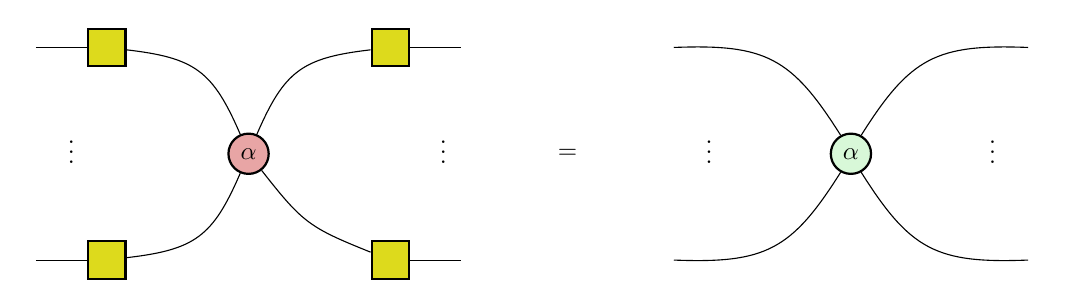
\begin{tikzpicture}[scale=0.9, every node/.style={scale=0.9}]
            \node [style=none] (0) at (-8, -1.5) {};
            \node [style=none] (1) at (-8, 1.5) {};
            \node [style=none] (2) at (-2, 1.5) {};
            \node [style=none] (3) at (-2, -1.5) {};
            \node [style=rn] (5) at (-5, 0) {\(\alpha\)};
            \node [style=had] (6) at (-7, -1.5) {};
            \node [style=had] (7) at (-7, 1.5) {};
            \node [style=had] (8) at (-3, 1.5) {};
            \node [style=had] (9) at (-3, -1.5) {};
            \node [style=none] (11) at (-0.5, 0) {\(=\)};
            \node [style=gn] (13) at (3.5, 0) {\(\alpha\)};
            \node [style=none] (14) at (6, 1.5) {};
            \node [style=none] (15) at (6, -1.5) {};
            \node [style=none] (16) at (1, -1.5) {};
            \node [style=none] (17) at (1, 1.5) {};
            \node [style=none] (18) at (-2.25, 0) {\(\rvdots\)};
            \node [style=none] (19) at (5.5, 0) {\(\rvdots\)};
            \node [style=none] (20) at (-7.5, 0) {\(\rvdots\)};
            \node [style=none] (21) at (1.5, 0) {\(\rvdots\)};
            \draw (0.center) to (6);
            \draw (1.center) to (7);
            \draw (8) to (2.center);
            \draw (9) to (3.center);
            \draw [bend right, looseness=1.25] (13) to (17.center);
            \draw [bend left, looseness=1.25] (13) to (16.center);
            \draw [bend right, looseness=1.25] (13) to (15.center);
            \draw [bend left, looseness=1.25] (13) to (14.center);
            \draw [bend right, looseness=1.25] (6) to (5);
            \draw [bend left, looseness=1.25] (7) to (5);
            \draw [bend left=15, looseness=1.25] (9) to (5);
            \draw [bend right, looseness=1.25] (8) to (5);
    \end{tikzpicture}    
\end{center}

Ta aksiom karakterizira Hadamardova vrata glede na to, kako spreminja pajke oziroma kako vpliva na preostanek diagrama, med tem ko prejšnji aksiom karakterizira vrata glede na to kaj vrata so na elementaren način, neodvisno od preostanka diagrama. Prejšnji opisuje kaj Hadamardova so, ta pa kaj naredijo.

\subsubsection{Eulerjevi koti} \label{euler} % http://www.pisrs.si/Pis.web/sodnaPraksaRSSearch?search=dodatek%20za%20pomo%C4%8D%20in%20postre%C5%BEbo&filter=&chosenFilters=visjeDelovno,upravno&od=&do=&page=4 prej naštetih je brez -
Zadnji aksiom je tudi najtežji in tudi najbolj nestandarden, vendar potreben za določene zaželjene lastnosti. Če imamo dva diagrama, katerima pripada enaka matrika, še ni nujno zagotovljeno, da obstaja zaporedje prej naštetih transformacij, ki prvega pretvori v drugega. Kot protiprimer služi ravno enakost v aksiomu Eulerjevih kotov. Če pa kot aksiom dodamo samo še to transformacijo, imamo zagotovljeno, da lahko poljubna diagrama, katerima pripada enaka matrika, preoblikujemo enega v drugega z uporabo aksiomov. To lastnost imenujemo \emph{polnost}.
\begin{center}
    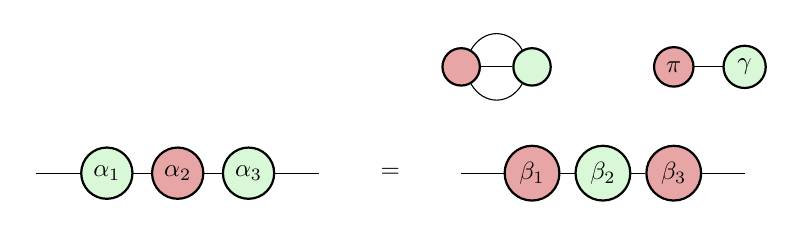
\begin{tikzpicture}[scale=0.9, every node/.style={scale=0.9}]
            \node [style=none] (0) at (-4, 0) {};
            \node [style=gn] (1) at (-3, 0) {\(\alpha_1\)};
            \node [style=gn] (2) at (-1, 0) {\(\alpha_3\)};
            \node [style=rn] (3) at (-2, 0) {\(\alpha_2\)};
            \node [style=none] (4) at (0, 0) {};
            \node [style=none] (5) at (1, 0) {\(=\)};
            \node [style=none] (6) at (2, 0) {};
            \node [style=none] (7) at (6, 0) {};
            \node [style=gn] (8) at (4, 0) {\(\beta_2\)};
            \node [style=rn] (9) at (5, 0) {\(\beta_3\)};
            \node [style=rn] (10) at (3, 0) {\(\beta_1\)};
            \node [style=rn] (11) at (2, 1.5) {};
            \node [style=gn] (12) at (3, 1.5) {};
            \node [style=rn] (13) at (5, 1.5) {\(\pi\)};
            \node [style=gn] (14) at (6, 1.5) {\(\gamma\)};
            \draw (0.center) to (1);
            \draw (1) to (3);
            \draw (3) to (2);
            \draw (2) to (4.center);
            \draw [bend left=60, looseness=1.25] (11) to (12);
            \draw [bend right=60, looseness=1.25] (11) to (12);
            \draw (11) to (12);
            \draw (13) to (14);
            \draw (6.center) to (10);
            \draw (10) to (8);
            \draw (8) to (9);
            \draw (9) to (7.center);
    \end{tikzpicture}    
\end{center}
Na levi strani enakosti imamo dane poljubne \(\alpha_1,\alpha_2,\alpha_3\), na desni strani pa moramo vrednosti izračunati. Definiramo si nekaj pomožnih vrednosti.
\begin{align*}
    x^+ &\defeq \frac{\alpha_1 + \alpha_3}{2}\\
    x^- &\defeq x^+-\alpha_3\\
    z &\defeq \cos\left(\frac{\alpha_2}{2}\right)\cos\left(x^+\right) + i\sin\left(\frac{\alpha_2}{2}\right)\cos\left(x^-\right)\\
    z' &\defeq \cos\left(\frac{\alpha_2}{2}\right)\sin\left(x^+\right) - i\sin\left(\frac{\alpha_2}{2}\right)\sin\left(x^-\right)
\end{align*}
Z njihovo pomočjo lahko izračunamo ostale parametre
\begin{align*}
    \beta_1 &= \arg z + \arg z'\\
    \beta_2 &= 2\arg\left(i+\left\lvert\frac{z}{z'}\right\rvert\right)\\
    \beta_3 &= \arg z - \arg z'\\
    \gamma &= x^+-\arg z + \frac{\alpha_2-\beta_2}{2}
\end{align*}
Po dogovoru vzamemo tako funkcijo \(\arg\), da \(\arg(0)=0\). Če je \(z'=0\) pa definiramo \(\beta_2 = 0\).

Motivacija za ta aksiom prihaja iz Eulerjevih kotov poznanih iz klasične analize. Te nam omogočijo dekompozicijo poljubne rotacije kot kompozicijo rotacij okoli standardnih koordinatnih osi. Enako lahko povemo v jeziku linearne algebre: poljubno rotacijsko matriko \(R\) lahko napišemo kot \(R=X(\alpha_1)Y(\alpha_2)Z(\alpha_3)\). Ta izrek ima v kvantni mehaniki pomembno posledico, namreč omogoča nam da lahko zapišemo poljuben unitarni operator enega kubita kot kompozicijo rotacij okoli \(Z,X,Z\) ali okoli \(X,Z,X\), ta aksiom pa nam definira, da sta dve dekompoziciji istega unitarnega operatorja ekvivalentni.

Ta aksiom je poseben tudi v tem, da so ostali aksiomi linearni, ta pa je nelinearen. To vidimo iz tega, da faze dobljenih pajkov niso linearne kombinacije ostalih faz, pač pa tukaj uporabimo tudi nelinearne kotne funkcije ter argument. Vendar pa je prav zato potreben za polnost jezika, saj je namreč znano, da različica ZX-računa brez nelinearnega aksioma ne more biti polna \cite[izrek 6.1]{jeandeldiagrammatic}.

\subsection{Primeri}
Za lažje razumevanje podanih aksiomov si poglejmo nekaj primerov in izrekov v ZX-računu, ki jih lahko dokažemo.

\emph{Inverz diagrama} \(D:n\to n\) je diagram \(D^{-1}:n\to n\), da \(D\circ D^{-1} = D^{-1}\circ D = \bigotimes_{i=1}^n\id\). Tukaj je identiteta \(\id\) samo povezava od vhoda do izhoda brez pajka; diagramu ustreza identična matrika \(\interpret{\bigotimes_{i=1}^n\id} = I = (\delta_{ij})_{i,j=1,\ldots 2^n}\). Že kot aksiom imamo podano to, da je pajek brez faze ekvivalenten identiteti, kar posledično pomeni, da je sam svoj inverz. Podobno velja tudi za Hadamardova vrata \(H\). Ta niso ekvivalentna identiteti, velja pa, da so svoj inverz \(H\circ H = \id\).
\begin{izrek}[Hadamard je sam sebi inverz]\label{had-inverz}
    Diagram
\begin{center}
    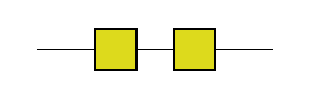
\begin{tikzpicture}
            \node [style=none] (0) at (-1, 0) {};
            \node [style=none] (1) at (2, 0) {};
            \node [style=had] (2) at (0, 0) {};
            \node [style=had] (3) at (1, 0) {};
            \draw (0.center) to (2);
            \draw (2) to (3);
            \draw (3) to (1.center);
    \end{tikzpicture}    
\end{center}
je ekvivalenten identiteti.
\end{izrek}
\begin{proof}

Uporabimo aksiom o identiteti \ref{identiteta}, ki pove, da je (prazna) povezava ekvivalentna povezavi s pajkom, ki ima fazo 0. To lahko uporabimo na povezavi med Hadamardovima vratoma, da vstavimo novega pajka in dobimo ekvivalentno vezje.
\begin{center}
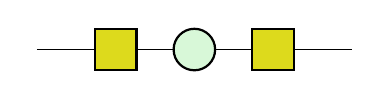
\begin{tikzpicture}
		\node [style=none] (0) at (-1, 0) {};
		\node [style=none] (1) at (3, 0) {};
		\node [style=had] (2) at (0, 0) {};
		\node [style=had] (3) at (2, 0) {};
		\node [style=gn] (4) at (1, 0) {};
		\draw (0.center) to (2);
		\draw (3) to (1.center);
		\draw (2) to (4);
		\draw (4) to (3);
\end{tikzpicture}
\end{center}
Temu sledi uporaba aksioma Hadamardove menjave barv \ref{had-menjava}.
\begin{center}
    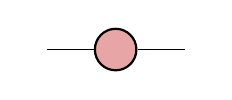
\begin{tikzpicture}
        \node [style=none] (0) at (0,0) {};
        \node [style=rn] (1) at (1,0) {};
        \node [style=none] (2) at (2,0) {};
        \draw (0) to (1);
        \draw (1) to (2);
    \end{tikzpicture}
\end{center}
Nazadnje spet uporabimo aksiom o identiteti \ref{identiteta}, kar nam poda identično preslikavo.
\begin{center}
    \begin{tikzpicture}
        \node [style=none] (0) at (0,0) {};
        \node [style=none] (2) at (2,0) {};
        \draw (0) to (2);
    \end{tikzpicture}
\end{center}
\end{proof}
Tako smo dokazali, da so Hadamardova vrata sama svoj inverz. Ta izrek lahko uporabimo v naslednjem primeru.
\begin{izrek}[Hadamard menja barve]\label{had-br}
    Velja enakost
\begin{center}
    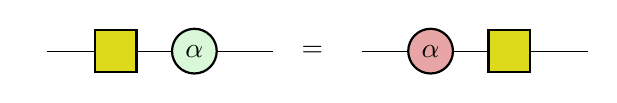
\begin{tikzpicture}
        \node (0) at (0, 0) {};
        \node [style=had] (h) at (1,0) {};
        \node [style=gn] (g) at (2,0) {\(\alpha\)};
        \node (0a) at (4, 0) {};
        \node (=) at (3.5,0) {\(=\)}; 
        \node [style=had] (ha) at (6,0) {};
        \node [style=rn] (ga) at (5,0) {\(\alpha\)};
        \draw (0) to (h);
        \draw (h) to (g);
        \draw (g) to (3,0);
        \draw (0a) to (ga);
        \draw (ha) to (ga);
        \draw (ha) to (7,0);
    \end{tikzpicture}.
\end{center}
\end{izrek}
\begin{proof}
Začnemo z levo stranjo enakosti in na njej uporabimo prejšnji izrek \ref{had-inverz}.
\begin{center}
    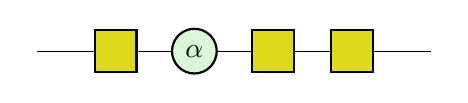
\begin{tikzpicture}
            \node [style=none] (0) at (-1, 0) {};
            \node [style=had] (2) at (0, 0) {};
            \node [style=gn] (4) at (1, 0) {\(\alpha\)};
            \node [style=had] (5) at (2, 0) {};
            \node [style=had] (6) at (3, 0) {};
            \node [style=none] (7) at (4, 0) {};
            \draw (0.center) to (2);
            \draw (2) to (4);
            \draw (4) to (5);
            \draw (5) to (6);
            \draw (6) to (7.center);
    \end{tikzpicture}    
\end{center}
Tako smo dobili diagram, na katerem lahko uporabimo Hadamardovo menjavo barv \ref{had-menjava}.
\begin{center}
    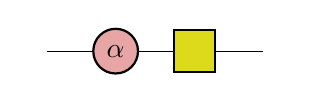
\begin{tikzpicture}
        \node [style=none] (0) at (0,0) {};
        \node [style=rn] (1) at (1,0) {\(\alpha\)};
        \node [style=had] (2) at (2,0) {};
        \node [style=none] (3) at (3,0) {};
        \draw (0) to (1);
        \draw (1) to (2);
        \draw (2) to (3);
    \end{tikzpicture}
\end{center}
\end{proof}

Zaključimo s Hopfovim zakonom, ki je teoretično zanimiv, saj nam omogoči, da povezan diagram pretvorimo v nepovezanega. Zaradi preglednosti pogosto skalarne diagrame pišemo manjše.
\begin{izrek}[Hopfov zakon] \label{hopf}
    Velja enakost
\begin{center}
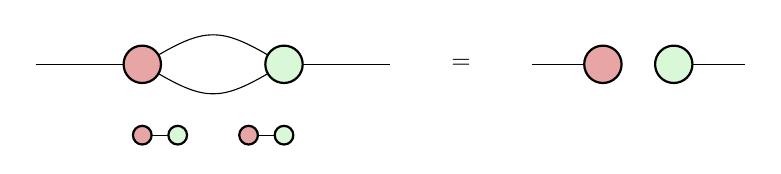
\begin{tikzpicture}[scale=0.9, every node/.style={scale=0.9}]
		\node [style=rn] (0) at (-0.5, 0) {};
		\node [style=rn, scale=0.5] (1) at (-0.5, -1) {};
		\node [style=rn, scale=0.5] (2) at (1, -1) {};
		\node [style=gn] (3) at (1.5, 0) {};
		\node [style=gn, scale=0.5] (4) at (0, -1) {};
		\node [style=gn, scale=0.5] (5) at (1.5, -1) {};
		\node [style=none] (6) at (-2, 0) {};
		\node [style=none] (7) at (3, 0) {};
		\node [style=none] (8) at (4, 0) {\(=\)};
		\node [style=none] (9) at (5, 0) {};
		\node [style=none] (10) at (8, 0) {};
		\node [style=rn] (11) at (6, 0) {};
		\node [style=gn] (12) at (7, 0) {};
		\draw [bend left, looseness=1.25] (0) to (3);
		\draw (1) to (4);
		\draw (2) to (5);
		\draw [bend right, looseness=1.25] (0) to (3);
		\draw (6.center) to (0);
		\draw (3) to (7.center);
		\draw (9.center) to (11);
		\draw (10.center) to (12);
\end{tikzpicture}.
\end{center}
\end{izrek}
\begin{proof}
Pravilo je posledica aksioma bialgebre \cite[poglavje 3.2.3]{Backens}. Začnemo na levi strani enakosti ter dvakrat uporabimo aksiom o identiteti \ref{identiteta}.
\begin{center}
    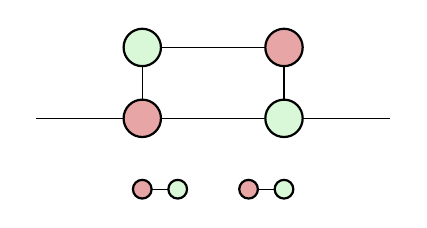
\begin{tikzpicture}[scale=0.9, every node/.style={scale=0.9}]
            \node [style=rn] (0) at (-0.5, 0) {};
            \node [style=rn, scale=0.5] (1) at (-0.5, -1) {};
            \node [style=rn, scale=0.5] (2) at (1, -1) {};
            \node [style=gn] (3) at (1.5, 0) {};
            \node [style=gn, scale=0.5] (4) at (0, -1) {};
            \node [style=gn, scale=0.5] (5) at (1.5, -1) {};
            \node [style=none] (6) at (-2, 0) {};
            \node [style=none] (7) at (3, 0) {};
            \node [style=rn] (8) at (1.5, 1) {};
            \node [style=gn] (9) at (-0.5, 1) {};
            \draw (1) to (4);
            \draw (2) to (5);
            \draw (0) to (3);
            \draw (6.center) to (0);
            \draw (3) to (7.center);
            \draw (9) to (0);
            \draw (9) to (8);
            \draw (8) to (3);
    \end{tikzpicture}    
\end{center}
Sedaj le topološko preuredimo diagram, da ima bolj znano obliko
\begin{center}
    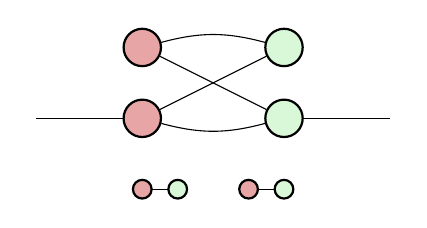
\begin{tikzpicture}[scale=0.9, every node/.style={scale=0.9}]
            \node [style=rn] (0) at (-0.5, 0) {};
            \node [style=rn, scale=0.5] (1) at (-0.5, -1) {};
            \node [style=rn, scale=0.5] (2) at (1, -1) {};
            \node [style=gn] (3) at (1.5, 0) {};
            \node [style=gn, scale=0.5] (4) at (0, -1) {};
            \node [style=gn, scale=0.5] (5) at (1.5, -1) {};
            \node [style=none] (6) at (-2, 0) {};
            \node [style=none] (7) at (3, 0) {};
            \node [style=rn] (8) at (-0.5, 1) {};
            \node [style=gn] (9) at (1.5, 1) {};
            \draw (1) to (4);
            \draw (2) to (5);
            \draw [bend right=15] (0) to (3);
            \draw (6.center) to (0);
            \draw (3) to (7.center);
            \draw (9) to (0);
            \draw [bend left=345] (9) to (8);
            \draw (8) to (3);
    \end{tikzpicture}    
\end{center}
Uporabimo aksiom o združitvi \ref{zdruzitev} v obratno smer -- že združena pajka (oba s fazo \(0\)) ločimo narazen. Novi pajek ne bo imel vhodov ali izhodov, le povezavo do drugega pajka, katerega je bil del.
\begin{center}
    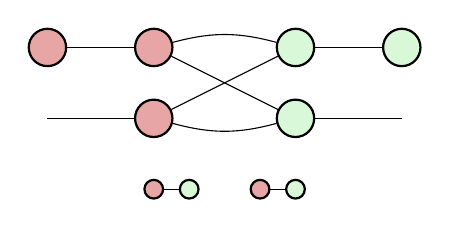
\begin{tikzpicture}[scale=0.9, every node/.style={scale=0.9}]
            \node [style=rn] (0) at (-0.5, 0) {};
            \node [style=rn, scale=0.5] (1) at (-0.5, -1) {};
            \node [style=rn, scale=0.5] (2) at (1, -1) {};
            \node [style=gn] (3) at (1.5, 0) {};
            \node [style=gn, scale=0.5] (4) at (0, -1) {};
            \node [style=gn, scale=0.5] (5) at (1.5, -1) {};
            \node [style=none] (6) at (-2, 0) {};
            \node [style=none] (7) at (3, 0) {};
            \node [style=rn] (8) at (-0.5, 1) {};
            \node [style=gn] (9) at (1.5, 1) {};
            \node [style=gn] (10) at (3, 1) {};
            \node [style=rn] (11) at (-2, 1) {};
            \draw (1) to (4);
            \draw (2) to (5);
            \draw [bend right=15] (0) to (3);
            \draw (6.center) to (0);
            \draw (3) to (7.center);
            \draw (9) to (0);
            \draw [bend left=345] (9) to (8);
            \draw (8) to (3);
            \draw (11) to (8);
            \draw (9) to (10);
    \end{tikzpicture}    
\end{center}
V temu diagramu pa prepoznamo aksiom bialgebre \ref{bialgebra}.
\begin{center}
    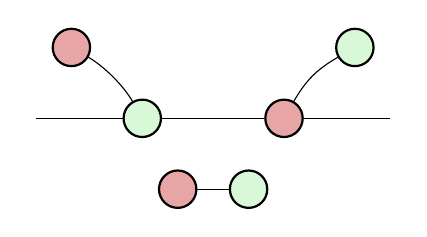
\begin{tikzpicture}[scale=0.9, every node/.style={scale=0.9}]
            \node [style=rn] (2) at (0, -1) {};
            \node [style=gn] (5) at (1, -1) {};
            \node [style=none] (6) at (-2, 0) {};
            \node [style=none] (7) at (3, 0) {};
            \node [style=gn] (8) at (-0.5, 0) {};
            \node [style=rn] (9) at (1.5, 0) {};
            \node [style=rn] (10) at (-1.5, 1) {};
            \node [style=gn] (11) at (2.5, 1) {};
            \draw (2) to (5);
            \draw (6.center) to (8);
            \draw (8) to (9);
            \draw (9) to (7.center);
            \draw [bend left=15, looseness=0.75] (10) to (8);
            \draw [bend right=15] (11) to (9);
    \end{tikzpicture}    
\end{center}
Diagram preuredimo
\begin{center}
    \begin{tikzpicture}[scale=0.9, every node/.style={scale=0.9}]
            \node [style=rn] (2) at (-2, 1) {};
            \node [style=gn] (5) at (-0.5, 1) {};
            \node [style=none] (6) at (0.5, -0.75) {};
            \node [style=none] (7) at (3, 0) {};
            \node [style=gn] (8) at (-0.5, 0) {};
            \node [style=rn] (9) at (1.5, 0) {};
            \node [style=rn] (10) at (-2, 0) {};
            \node [style=gn] (11) at (2.5, 1) {};
            \node [style=none] (12) at (-2, -1) {};
            \draw (2) to (5);
            \draw [in=-45, out=90, looseness=0.75] (6.center) to (8);
            \draw [bend left=15] (8) to (9);
            \draw (9) to (7.center);
            \draw (10) to (8);
            \draw [bend right=15] (11) to (9);
            \draw [in=-90, out=0, looseness=0.75] (12.center) to (6.center);
    \end{tikzpicture}
\end{center}
in uporabimo pravilo kopiranja \ref{kopiranje}.
\begin{center}
    \begin{tikzpicture}[scale=0.9, every node/.style={scale=0.9}]
            \node [style=none] (7) at (3, 0) {};
            \node [style=rn] (9) at (1.5, 0) {};
            \node [style=gn] (11) at (2.5, 1) {};
            \node [style=none] (12) at (-2, 0) {};
            \node [style=rn] (13) at (-1, 0) {};
            \node [style=rn] (14) at (0, 0) {};
            \draw (9) to (7.center);
            \draw [bend right=15] (11) to (9);
            \draw (12.center) to (13);
            \draw (14) to (9);
    \end{tikzpicture}    
\end{center}
Pajke lahko združimo (aksiom \ref{zdruzitev}) in poenostavimo z izbrisom identitet (aksiom \ref{identiteta}), kar dokaže lastnost.
\begin{center}
    \begin{tikzpicture}
        \node [style=none] (0) at (0,0) {};
        \node [style=rn] (1) at (1,0) {};
        \node [style=gn] (2) at (2,0) {};
        \node [style=none] (3) at (3,0) {};
        \draw (0) to (1);
        \draw (2) to (3);
    \end{tikzpicture}
\end{center}
\end{proof}
Za intuicijo zakona sledimo toku podatkov. Na levi strani enačbe imamo povezavo od pajka X do pajka Z, na desni strani enačbe pa vhod pride do pajka X, se pozabi, pajek Z pa se na novo (neodvisno) izmisli nove podatke, ter jih pošlje naprej. To je posledica tega, da sta pajka X in Z v različni bazi -- če najprej izmerimo spin v X smeri in potem v Z smeri smo izgubili prvotno informacijo \cite[definicija 8.27]{coecke_kissinger_2017}. V praksi pa nam dovoli, da razbijemo povezan diagram na nepovezane dele in ga tako poenostavimo.

Hopfov zakon lahko uporabimo tudi, če ima pajek več vhodov ali izhodov, saj lahko vezje oblike
\begin{center}
    \begin{tikzpicture}[scale=0.9, every node/.style={scale=0.9}]
            \node [style=rn] (0) at (-2, 0) {};
            \node [style=gn] (1) at (0, 0) {};
            \node [style=none] (2) at (2, 0) {\(\rvdots\)};
            \node [style=none] (3) at (-4, 0) {\(\rvdots\)};
            \node [style=none] (4) at (-4, 1) {};
            \node [style=none] (5) at (-4, -1) {};
            \node [style=none] (6) at (2, -1) {};
            \node [style=none] (7) at (2, 1) {};
            \node [style=rn, scale=0.5] (8) at (-2, 1) {};
            \node [style=rn, scale=0.5] (9) at (-0.5, 1) {};
            \node [style=gn, scale=0.5] (10) at (-1.5, 1) {};
            \node [style=gn, scale=0.5] (11) at (0, 1) {};
            \draw [bend left=15] (4.center) to (0);
            \draw [bend right=15] (5.center) to (0);
            \draw [bend right=15] (7.center) to (1);
            \draw [bend right=15] (1) to (6.center);
            \draw [bend left] (0) to (1);
            \draw [bend right] (0) to (1);
            \draw (8) to (10);
            \draw (9) to (11);
    \end{tikzpicture}     
\end{center}
prepišemo v vezje
\begin{center}
    \begin{tikzpicture}[scale=0.9, every node/.style={scale=0.9}]
            \node [style=rn] (0) at (-2, 0) {};
            \node [style=gn] (1) at (2, 0) {};
            \node [style=none] (2) at (3.75, 0) {\(\rvdots\)};
            \node [style=none] (3) at (-4, 0) {\(\rvdots\)};
            \node [style=none] (4) at (-4, 1) {};
            \node [style=none] (5) at (-4, -1) {};
            \node [style=none] (6) at (3.75, -1) {};
            \node [style=none] (7) at (3.75, 1) {};
            \node [style=rn] (8) at (-1, 0) {};
            \node [style=gn] (9) at (1, 0) {};
            \node [style=rn, scale=0.5] (10) at (-1, 1) {};
            \node [style=rn, scale=0.5] (11) at (0.5, 1) {};
            \node [style=gn, scale=0.5] (12) at (-0.5, 1) {};
            \node [style=gn, scale=0.5] (13) at (1, 1) {};
            \draw [bend left=15] (4.center) to (0);
            \draw [bend right=15] (5.center) to (0);
            \draw [bend right=15] (7.center) to (1);
            \draw [bend right=15] (1) to (6.center);
            \draw (0) to (8);
            \draw (9) to (1);
            \draw [bend right=330] (9) to (8);
            \draw [bend left] (8) to (9);
            \draw (10) to (12);
            \draw (11) to (13);
    \end{tikzpicture}     
\end{center}
z uporabo aksioma združitve \ref{zdruzitev}, kar pa je oblika diagrama, ki ustreza Hopfovem zakonu.
\subsection{Lastnosti}
Da upravičimo uporabo ZX-računa, želimo nekaj dobrih lastnosti. Že prej smo omenili polnost jezika, obstaja pa še nekaj ostalih temeljnih lastnosti, katerih si želimo. Najbolj osnovna lastnost je skladnost.
\subsubsection{skladnost}
\begin{izrek}[skladnost]
    Če lahko diagram \(D_1:n\to m\) prepišemo v \(D_2:n\to m\) z uporabo aksiomov ZX-računa, potem \(\interpret{D_1} = \interpret{D_2}\).
\end{izrek}
Ta izrek enostavno preverimo tako, da pretvorimo leve in desne strani vsake enakosti podane v aksiomih v matriko ter vidimo, da se ujemajo \cite[izrek 2.16]{Coecke_2011}.

Skladnost je predpogoj za uporabo katere koli teorije. Ne glede na to kako lepe lastnosti ima teorija, če se ne strinja z originalno, pravo, različico ni uporabna.

Tukaj velja še omeniti skalarne diagrame. Mnogi pristopi v aksiomih izpustijo skalarne diagrame, vendar v tem primeru skladnost ne velja. To sicer nima velikega praktičnega pomena, saj skladnost še vedno velja do skalarja natančno, zaradi unitarnosti kvantnih preslikav pa ne izgubimo veliko informacij zaradi skalarjev. V tem primeru delamo z ekvivalenčnimi razredi matrik.
\subsubsection{Polnost}
\begin{izrek}[Polnost]
    Če imamo dva diagrama \(D_1:n\to m\) in \(D_2:n\to m\), za katera velja \(\interpret{D_1} = \interpret{D_2}\), potem lahko \(D_1\) pretvorimo v \(D_2\) (ali obratno) z uporabo aksiomov.
\end{izrek}
Že od samega začetka uvedbe ZX-računa je bila polnost najbolj iskana lastnost jezika. Dovoli namreč, da lahko vsako lastnost, ki drži v Diracovem formalizmu, dokažemo tudi v ZX-računu, kar pa ne velja z uporabo klasičnih vezij, saj za njih nimamo dovolj močnih pravil poenostavljanj. Prvotne izbire aksiomov niso bile polne, kar je omejilo ekspresivnost jezika in možnost njegove uporabe. Večina formalizacij je potrebovala nekakšen nelinearen aksiom, pri nas pa za to poskrbi aksiom Eulerjevih kotov \ref{euler}. Že pri zgodnjih rezultatih so sumili, da je podoben aksiom potreben \cite{Schr_der_de_Witt_2014}, vendar ni bilo znano, ali je zadosten. Kasneje pa so dokazali, da je bila to edina večja prepreka in leta 2017 dokazali polnost. Dokaz polnosti je potekal preko podobnega grafičnega jezika ZW-računa, za katerega je bila polnost že znana \cite{kangfengng}.

Oglejmo si primer uporabe polnosti.
\begin{primer}[Inverz korena]\label{inv-koren}
    Vezje
    \begin{center}
        \begin{tikzpicture}[scale=0.9, every node/.style={scale=0.9}]
                \node [style=gn] (0) at (-1, 0) {};
                \node [style=rn] (1) at (1, 0) {};
                \node [style=gn] (2) at (-1, 1) {};
                \node [style=rn] (3) at (1, 1) {};
                \draw (0) to (1);
                \draw [bend right=45] (0) to (1);
                \draw [bend left=45] (0) to (1);
                \draw (2) to (3);
        \end{tikzpicture}        
    \end{center}
    je ekvivalentno praznemu diagramu.
    
    Ker je diagram sestavljen iz dveh komponent, je njegova interpretacija teznorski produkt obeh povezanih komponent. Obe komponenti sta skalarna diagrama, kar pomeni, da predstavljata števili. Izračunamo kateri števili predstavljata, ter preverimo, da sta res inverzni za množenje (saj je tenzorski produkt \(1\times 1\) matrik kar množenje).

    Za vrednost zgornje komponente smo že izračunali v primeru \ref{skal}, da je enaka \(\sqrt{2}\).
    Za spodnjo komponento si najprej izračunamo vrednosti elementarnih stanj. To izračunamo po definiciji tenzorskega produkta in zapisa \(\bra{xxx} = \bra{x}\otimes \bra{x}\otimes \bra{x}\). Izračunamo le braje \(\bra{\cdot}\), saj so keti le transponirani braji \(\ket{x}=\bra{x}^\tranp\).
    \begin{align*}
        \bra{000} = \begin{bmatrix}
            1&0&0&0& 0&0&0&0
        \end{bmatrix}\\
        \bra{111} = \begin{bmatrix}
            0&0&0&0& 0&0&0&1
        \end{bmatrix}\\
        \bra{+++} = \frac{1}{2\sqrt{2}}\begin{bmatrix}
            1&1&1&1& 1&1&1&1
        \end{bmatrix}\\
        \bra{---} = \frac{1}{2\sqrt{2}} \begin{bmatrix}
            1&-1&-1&1& -1&1&1&-1
        \end{bmatrix}
    \end{align*}
    Sedaj pretvorimo vezje v račun
    \begin{align*}
        (\bra{+++}+\bra{---})(\ket{000}+\ket{111})=\\
        =\braket{+++}{000}+\braket{+++}{111}+\braket{---}{000}+\braket{---}{111}\\
        =\frac{1}{2\sqrt2}+\frac{1}{2\sqrt2}+\frac{1}{2\sqrt2}-\frac{1}{2\sqrt2}\\
        =\frac{1}{\sqrt2}
    \end{align*}
    Očitno je \(\sqrt2/\sqrt2 = 1\), kar pa je prazni diagram. Torej imata oba diagrama enako interpretacijo in sta, po polnosti, ekvivalentna v ZX-računu.
\end{primer}
Ta pristop običajno ni uporaben. Že v primeru skalarnih diagramov na treh kubitih imamo opravka z vektorji z osmimi elementi. V kvantnih vezjih je običajno enako število vhodov kot izhodov, torej bi imeli opravka z \(8\times8\) matriko. Ob času pisanja ima najzmoglivejši kvantni računalnik \(127\) kubitov \cite{hugh}, kar je za veliko uporab še vedno premalo. Če bi želeli napisati matriko, ki predstavlja vezje takega računalnika bi dobili \(2^{127}\times 2^{127}\) matriko, kar je praktično neizračunljivo. Če pa se držimo ZX-diagramov pa ima vezje 127 vhodnih in 127 izhodnih povezav. Tako ima pri polnosti večji pomen to, da zagotovi, da vezje lahko poenostavimo, kot pa to, da preverjamo enakost z matrikami.
\subsubsection{Univerzalnost}
Vemo že, da vsakemu diagramu pripada neka matrika. Velja pa tudi obratno in vsaki matriki pripada nek diagram.
\begin{izrek}[Univerzalnost]
    Za poljubno linearno preslikavo kubitov \(A:\C^{2^n}\to \C^{2^m}\), ki preslika \(n\) kubitov v \(m\) kubitov, obstaja ZX-diagram \(D:n\to m\) za katerega velja \(\interpret{D}=A\).
\end{izrek}
\begin{proof}
Vemo, da lahko poljubno unitarno preslikavo \(n\) kubitov napišemo z uporabo \textsf{cNOT} vrat ter eno kubitnih unitarnih preslikav \cite[Izrek 5.26]{mathforqm}. Če to naredimo, je potreben le postopek pretvarjanja \textsf{cNOT} vrat v ZX-račun in pretvarjanja splošnih enokubitnih unitarnih preslikav v ZX-račun. Vemo, da \textsf{cNOT} vratom pripada matrika
\begin{align*}
    \begin{bmatrix}
        1&0&0&0\\
        0&1&0&0\\
        0&0&0&1\\
        0&0&1&0
    \end{bmatrix}.
\end{align*}
Interpretacija diagrama
\begin{center}
    \begin{tikzpicture}[scale=0.9, every node/.style={scale=0.9}]
            \node [style=gn] (fixg) at (-0.5, -1) {};
            \node [style=rn] (fixr) at (0.5, -1) {}; 
            \node [style=gn] (0) at (0, 1) {};
            \node [style=rn] (1) at (0, 0) {};
            \node [style=none] (2) at (-1, 1) {};
            \node [style=none] (3) at (-1, 0) {};
            \node [style=none] (4) at (1, 1) {};
            \node [style=none] (5) at (1, 0) {};
            \draw (2.center) to (0);
            \draw (0) to (4.center);
            \draw (3.center) to (1);
            \draw (1) to (5.center);
            \draw (0) to (1);
            \draw (fixg) to (fixr);
    \end{tikzpicture}  
\end{center}
pa je ravno ta matrika. Poljubno unitarno preslikavo enega kubita pa lahko napišemo kot kompozitum Eulerjevih kotov \cite[Izrek 5.11]{mathforqm}. Pajki sami pa po definiciji ustrezajo rotacijam okoli X in Z osi. Torej lahko poljubno unitarno preslikavo napišemo kot
\begin{center}
    \begin{tikzpicture}
        \node [style=none] (0) at (0,0) {};
        \node [style=gn] (1) at (1,0) {\(\alpha\)};
        \node [style=rn] (2) at (2,0) {\(\beta\)};
        \node [style=gn] (3) at (3,0) {\(\gamma\)};
        \node [style=none] (4) at (4,0) {};
        \draw (0) to (1) to (2) to (3) to (4);
    \end{tikzpicture}.
\end{center}
Sedaj imamo univerzalnost za unitarne preslikave \(n\) kubitov v \(n\) kubitov. Kvantna stanja dobimo kot sliko takšne preslikave; za poljubno željeno kvantno stanje \(n+m\) kubitov po univerzalnosti obstaja ZX-diagram, ki vhod \(n+m\) zelenih pajkov preslika v to stanje. Diagram, ki to predstavlja, je \(n+m\) zelenih pajkov, ki vodijo v preostanek diagrama, ven iz diagrama pa vodi \(n+m\) povezav. Zaradi topološke ekvivalence diagramov pa ni razlike med \(n+m\) izhodi ter \(n\) vhodi in \(m\) izhodi, saj lahko \(n\) izhodnih povezav prestavimo, da iz diagrama izhajajo na levo in obratno. Tako željeno preslikavo, ki sprejme \(n\) kubitov, odda pa jih \(m\), pretvorimo v iskanje kvantnega stanja \(n+m\) kubitov (za kar vemo, da obstaja diagram), potem pa to stanje nazaj pretvorimo (spet z uporabo topološke ekvivalence) v \(D:n\to m\) diagram, kar dokaže univerzalnost \cite[Izrek 2.18]{Coecke_2011}. \end{proof}

Izrek o univerzalnosti nam pove, da so diagrami dovolj ekspresivni in lahko opišejo poljubno transformacijo kubitov. Izrek o polnosti pa nam pove, da niso \emph{preveč} ekspresivni in bi lahko neko transformacijo opisali na več neekvivalentnih načinov. Če združimo izreka skupaj dobimo, da lahko vsako kvantno transformacijo napišemo na natanko en način, do pravil prepisovanja natančno.

\subsection{Različice}
\emph{Različica} ZX-računa je formalizem, kjer omejimo konstrukcije v diagramu, navadno dovoljene faze pajkov. Tako v primeru \(\frac\pi2\) različice namesto \(\alpha\in \R\), uporabimo le \(\alpha\in\{k\cdot \frac\pi2\mid k\in\Z\}\). Različice imajo posebaj pomembno zgodovinsko vlogo, saj so za njih polnost jezika dokazali pred polnostjo splošnega ZX-računa.
\subsubsection{Različica Cliffordove teorije}
Tu dovolimo le faze, ki so večkratniki števila \(\frac\pi2\). Ta različica ustreza Cliffordovi kvantni mehaniki. Dovoljene so samo meritve, priprave stanj in unitarne transformacije, ki so del Cliffordove grupe.
\begin{definicija}
    \emph{Paulijeva grupa} \(n\) kubitov \(P_n\) je grupa tenzorskih produktov Paulijevih matrik
    \begin{align*}
        P_n = \left\{\alpha g_1\otimes g_2\otimes\cdots\otimes g_n \mid \alpha\in\{\pm 1, \pm i\}, \forall k\in\{1,\ldots n\}\sep g_k\in \{I,X,Y,Z\}\right\},
    \end{align*}
    kjer so Paulijeve matrike \(X,Y,Z\) standardne kot v definiciji \ref{Pauli}, \(I\) pa predstavlja identično matriko.
\end{definicija}
\begin{definicija}
    \emph{Cliffordova grupa} \(n\) kubitov \(C_n\) je grupa operatorjev \[C_n=\{U\mid \forall g\in P_n\sep UgU^\tranp\in P_n\}\] z operacijo množenja.
\end{definicija}
Pogosto uporabljen izraz je tudi stabilizatorska kvantna mehanika, saj po definiciji, če unitarni operator stabilizira \(\ket \psi\), potem velja \(U\ket\psi = \ket\psi\). Kvantno stanje je stabilizatorsko, če ga stabilizirajo Paulijeve matrike (za več-kubitno verzijo vzamemo tenzorske produkte Paulijevih matrik) \cite{Backens1}. Cliffordova grupa pa je grupa unitarnih operatorjev, ki preslikajo stabilizatorska stanja v stabilizatorska. Če bi faze omejili na \(\pi\Z\), pa bi opisovali realno stabilizatorsko kvantno mehaniko.

Polnost različice za stabilizatorsko kvantno mehaniko so dokazali že leta 2013 \cite{Backens1}. Na žalost ima stabilizatorska kvantna mehanika mnogo pomankljivosti. Kljub temu, da je uporabna za popravilo napak in določene modele kvantnega računanja, različica ni univerzalna in torej ne more predstavljati vseh algoritmov ali izrekov kvantne mehanike. Še huje, vsako stabilizatorsko kvantno vezje lahko učinkovito simuliramo na klasičnem računalniku \cite{Aaronson_2004}. To pa pomeni, da nam dodatek Cliffordove kvantne mehanike v računalništvo ne pomaga znatno, saj bi vsak algoritem lahko izvedli tudi brez vpletanja kvantnih algoritmov. Na srečo izrek o učinkoviti simulaciji ne velja za bolj drobno porazdeljene faze.
\subsubsection{Različica enokubitne Clifford+T teorije}
Tu dovolimo le faze, ki so večkratniki števila \(\frac\pi4\), operiramo pa samo na enem kubitu. To pomeni, da ima vsak pajek eno vhodno povezavo ter eno izhodno povezavo. Ta različica ustreza Cliffordovi+T kvantni mehaniki na enem kubitu. Polnost te različice so dokazali leta 2014 \cite{backens2014zx}, pomembna pa je, saj je prva različica, ki je dovolj močna, da opisuje prave kvantne procese. Sicer različica ni zmožna opisovati procesov več kubitov, niti ni zmožna točno opisovati kvantnih operacij nad enim kubitom, lahko pa do poljubne natančnosti opiše kvantne procese enega kubita \cite{814621}. Natančno ne more simulirati faz, ki so iracionalni večkratniki števila \(\pi\), lahko se pa tej fazi poljubno približamo.
\subsubsection{Različica Clifford+T teorije}
Različica, ki opisuje Clifford+T teorijo ima dovoljene le faze, ki so celoštevilski večkratniki \(\frac\pi4\). Za razliko od enokubitne različice dovoljuje poljubno število vhodnih in izhodnih povezav v pajke. Podobno kot enokubitna različica lahko ta opiše kvantne procese do poljubne natančnosti, dovoljuje pa tudi uporabo večjega števila kubitov. Polnost te različice je bila dokazana leta 2018 \cite{SimonCompleteness} vendar se dokaz polnosti splošnega jezika nanaša na ta rezultat, kljub temu, da je bil članek objavljen že leta 2017 \cite{kangfengng}.
\section{Uporaba ZX-diagramov}
\subsection{Poenostavljanje kvantnih vezij}
Ena izmed bolj pomembnih uporab ZX-računa je iskanje bolj enostavnih kvantnih vezij. Ponavadi imamo vezje napisano s klasični diagrami, ki opisujejo nek algoritem, želimo pa taisti algoritem napisati z manjšim številom vrat. To lahko naredimo tako, da vezje napišemo v ZX-računu in ga poenostavimo, potem pa pretvorimo nazaj v običajno kvantno vezje. Poglejmo si enostaven primer.
\begin{izrek}
    Vezje
    \begin{center}
        \begin{tikzpicture}
            \node[scale=1.0] {
              \begin{quantikz}
                \qw & \ctrl{1}  & \gate[swap]{} & \qw \\
                \qw & \targ{}   &               & \qw
              \end{quantikz}
            };
        \end{tikzpicture}
    \end{center}
    je ekvivalentno vezju
    \begin{center}
        \begin{tikzpicture}
            \node[scale=1.0] {
              \begin{quantikz}
                \qw & \gate[swap]{} & \targ{}  & \qw \\
                \qw &               & \ctrl{-1} & \qw
              \end{quantikz}
            };
        \end{tikzpicture}
    \end{center}.
\end{izrek}
\begin{proof}
    Vezje pretvorimo v ZX-diagram
    \begin{center}
        \begin{tikzpicture}[scale=0.9, every node/.style={scale=0.9}]
            \node [style=none] (14) at (-2, 1) {};
            \node [style=none] (15) at (-2, -1) {};
            \node [style=none] (18) at (1, -1) {};
            \node [style=none] (19) at (1, 1) {};
            \node [style=none] (20) at (2, 1) {};
            \node [style=none] (21) at (2, -1) {};
            \node [style=gn] (24) at (-1, 1) {};
            \node [style=rn] (25) at (-1, -1) {};
            \node [style=rn] (26) at (-1, 2) {};
            \node [style=gn] (27) at (1, 2) {};
            \draw (19.center) to (20.center);
            \draw (18.center) to (21.center);
            \draw [in=0, out=180] (18.center) to (24);
            \draw (24) to (14.center);
            \draw (15.center) to (25);
            \draw [in=-180, out=0, looseness=0.75] (25) to (19.center);
            \draw (24) to (25);
            \draw (26) to (27);
        \end{tikzpicture}
    \end{center}
    in ga topološko preuredimo
    \begin{center}
        \begin{tikzpicture}[scale=0.9, every node/.style={scale=0.9}]
            \node [style=none] (14) at (-2, 1) {};
            \node [style=none] (15) at (-2, -1) {};
            \node [style=none] (b1) at (-3, 1) {};
            \node [style=none] (b2) at (-3, -1) {};
            \node [style=none] (18) at (1, -1) {};
            \node [style=none] (19) at (1, 1) {};
            \node [style=gn] (24) at (0, -1) {};
            \node [style=rn] (25) at (0, 1) {};
            \node [style=rn] (26) at (-2, 2) {};
            \node [style=gn] (27) at (0, 2) {};
            \draw (b1) to (14.center);
            \draw (b2) to (15.center);
            \draw [in=0, out=180] (18.center) to (24);
            \draw [in=0, out=-180, looseness=0.75] (24) to (14.center);
            \draw [in=-180, out=0, looseness=0.75] (15.center) to (25);
            \draw [in=-180, out=0, looseness=0.75] (25) to (19.center);
            \draw (24) to (25);
            \draw (26) to (27);
        \end{tikzpicture}.
    \end{center}
    Ob tej točki lahko diagram enostavno pretvorimo nazaj v kvantno vezje.
\end{proof}
Izrek je sicer uporaben ter pokaže moč topološke ekvivalence diagramov, vendar ne pokaže polne moči aksiomov ZX-računa.
\begin{izrek}[\textsf{cNOT} dekompozicija \textsf{swap} \protect{\cite[Primer 4.2]{peham}}] \label{swap-dekomp}
    Vezje 
    \begin{center}
        \begin{tikzpicture}
            \node[scale=1.0] {
              \begin{quantikz}
                \qw & \ctrl{1}  & \targ{} & \ctrl{1} & \qw \\
                \qw & \targ{}  & \ctrl{-1} & \targ{}  & \qw
              \end{quantikz}
            };
          \end{tikzpicture}
        \end{center}
        je ekvivalentno vezju 
        \begin{center}
            \begin{tikzpicture}
                \node {
                    \begin{quantikz}
                        \qw &  \gate[swap]{} & \qw \\
                        \qw &  & \qw
                      \end{quantikz}
                    };
            \end{tikzpicture}.
        \end{center}
\end{izrek}
\begin{proof}
    Pretvorimo prvotno vezje v ZX-diagram.
    \begin{center}
        \begin{tikzpicture}[scale=0.9, every node/.style={scale=0.9}]
                \node [style=gn] (0) at (-2, 1) {};
                \node [style=gn] (1) at (-1, -1) {};
                \node [style=gn] (2) at (0, 1) {};
                \node [style=rn] (3) at (-2, -1) {};
                \node [style=rn] (4) at (-1, 1) {};
                \node [style=rn] (5) at (0, -1) {};
                \node [style=rn, scale=0.5] (6) at (-2, 1.7) {};
                \node [style=rn, scale=0.5] (7) at (-1, 1.7) {};
                \node [style=rn, scale=0.5] (8) at (0, 1.7) {};
                \node [style=gn, scale=0.5] (9) at (-2, 2.2) {};
                \node [style=gn, scale=0.5] (10) at (-1, 2.2) {};
                \node [style=gn, scale=0.5] (11) at (0, 2.2) {};
                \node [style=none] (12) at (1, 1) {};
                \node [style=none] (13) at (1, -1) {};
                \node [style=none] (14) at (-3, 1) {};
                \node [style=none] (15) at (-3, -1) {};
                \draw (0) to (4);
                \draw (4) to (2);
                \draw (2) to (12.center);
                \draw (14.center) to (0);
                \draw (15.center) to (3);
                \draw (3) to (1);
                \draw (1) to (5);
                \draw (5) to (13.center);
                \draw (5) to (2);
                \draw (4) to (1);
                \draw (0) to (3);
                \draw (9) to (6);
                \draw (10) to (7);
                \draw (11) to (8);
        \end{tikzpicture}       
    \end{center}
    Vezje topološko preuredimo.
    \begin{center}
        \begin{tikzpicture}[scale=0.9, every node/.style={scale=0.9}]
                \node [style=gn] (0) at (-3.75, 1) {};
                \node [style=gn] (1) at (-1.5, 1) {};
                \node [style=gn] (2) at (0, 1) {};
                \node [style=rn] (3) at (-3.75, -1) {};
                \node [style=rn] (4) at (-1.5, -1) {};
                \node [style=rn] (5) at (0, -1) {};
                \node [style=rn] (6) at (-2.25, 1) {};
                \node [style=gn] (9) at (-2.25, -1) {};
                \node [style=rn, scale=0.5] (7) at (-3.75, 2.5) {};
                \node [style=rn, scale=0.5] (8) at (-0.75, 2.5) {};
                \node [style=gn, scale=0.5] (10) at (-3.75, 3) {};
                \node [style=gn, scale=0.5] (11) at (-0.75, 3) {};
                \node [style=none] (12) at (1, 1) {};
                \node [style=none] (13) at (1, -1) {};
                \node [style=none] (14) at (-4.75, 1) {};
                \node [style=none] (15) at (-4.75, -1) {};
                \node [style=none] (17) at (2, 1) {};
                \node [style=none] (18) at (2, -1) {};
                \draw [in=-90, out=-75, looseness=2.00] (0) to (4);
                \draw (4) to (2);
                \draw [in=105, out=90, looseness=3.25] (2) to (12.center);
                \draw (14.center) to (0);
                \draw (15.center) to (3);
                \draw [in=90, out=75, looseness=2.25] (3) to (1);
                \draw (1) to (5);
                \draw [in=-105, out=-90, looseness=3.25] (5) to (13.center);
                \draw (5) to (2);
                \draw (4) to (1);
                \draw (0) to (3);
                \draw (9) to (6);
                \draw (10) to (7);
                \draw (11) to (8);
                \draw [in=180, out=-75, looseness=1.25] (12.center) to (17.center);
                \draw [in=180, out=75, looseness=1.25] (13.center) to (18.center);
        \end{tikzpicture}  
    \end{center}
    Na temu vezju pa lahko uporabimo aksiom bialgebre \ref{bialgebra}. Nato ga še topološko preuredimo. 
    \begin{center}
        \begin{tikzpicture}[scale=0.9, every node/.style={scale=0.9}]
                \node [style=gn] (0) at (-2.25, 1) {};
                \node [style=rn] (3) at (-2.25, -1) {};
                \node [style=rn, scale=0.5] (7) at (-2.25, 1.7) {};
                \node [style=rn, scale=0.5] (8) at (-1.25, 1.7) {};
                \node [style=gn, scale=0.5] (10) at (-2.25, 2.2) {};
                \node [style=gn, scale=0.5] (11) at (-1.25, 2.2) {};
                \node [style=none] (14) at (-3, 1) {};
                \node [style=none] (15) at (-3, -1) {};
                \node [style=rn] (16) at (-1.25, -1) {};
                \node [style=gn] (17) at (-1.25, 1) {};
                \node [style=none] (18) at (1, -1) {};
                \node [style=none] (19) at (1, 1) {};
                \node [style=none] (20) at (2, 1) {};
                \node [style=none] (21) at (2, -1) {};
                \draw (14.center) to (0);
                \draw (15.center) to (3);
                \draw (0) to (3);
                \draw (10) to (7);
                \draw (11) to (8);
                \draw (0) to (17);
                \draw (17) to (16);
                \draw (16) to (3);
                \draw [in=-180, out=-45] (17) to (18.center);
                \draw [in=-180, out=45] (16) to (19.center);
                \draw (19.center) to (20.center);
                \draw (18.center) to (21.center);
        \end{tikzpicture}        
    \end{center}
    Sosednja pajka združimo (aksiom \ref{zdruzitev}), kar da dvojno povezavo med pajkoma Z in X. To omogoči uporabo Hopfovega zakona \ref{hopf}, kar uporabi še preostala dva skalarna diagrama.
    \begin{center}
        \begin{tikzpicture}[scale=0.9, every node/.style={scale=0.9}]
                \node [style=none] (14) at (-3, 1) {};
                \node [style=none] (15) at (-3, -1) {};
                \node [style=rn] (16) at (-1.25, -1) {};
                \node [style=gn] (17) at (-1.25, 1) {};
                \node [style=none] (18) at (1, -1) {};
                \node [style=none] (19) at (1, 1) {};
                \node [style=none] (20) at (2, 1) {};
                \node [style=none] (21) at (2, -1) {};
                \draw [in=-180, out=-45] (17) to (18.center);
                \draw [in=-180, out=45] (16) to (19.center);
                \draw (19.center) to (20.center);
                \draw (18.center) to (21.center);
                \draw (14.center) to (17);
                \draw (15.center) to (16);
        \end{tikzpicture}        
    \end{center}
    Z uporabo aksioma identitete \ref{identiteta} dobimo vezje, ki ustreza vratom \textsf{swap}
    \begin{center}
        \begin{tikzpicture}[scale=0.9, every node/.style={scale=0.9}]
                \node [style=none] (14) at (-2, 1) {};
                \node [style=none] (15) at (-2, -1) {};
                \node [style=none] (18) at (1, -1) {};
                \node [style=none] (19) at (1, 1) {};
                \node [style=none] (20) at (2, 1) {};
                \node [style=none] (21) at (2, -1) {};
                \node [style=none] (22) at (-1, 1) {};
                \node [style=none] (23) at (-1, -1) {};
                \draw (19.center) to (20.center);
                \draw (18.center) to (21.center);
                \draw [in=-180, out=0, looseness=0.75] (22.center) to (18.center);
                \draw [in=0, out=180, looseness=0.75] (19.center) to (23.center);
                \draw (14.center) to (22.center);
                \draw (15.center) to (23.center);
        \end{tikzpicture}.
    \end{center}
\end{proof}
Dokažemo še podoben izrek z dvemi \textsf{cNOT} vrati.
\begin{izrek}[\textsf{cNOT} je svoj inverz] \label{cnot-inverse}
    Vezje 
    \begin{center}
        \begin{tikzpicture}
            \node[scale=1.0] {
              \begin{quantikz}
                \qw & \ctrl{1} & \ctrl{1} & \qw \\
                \qw & \targ{}  & \targ{}  & \qw
              \end{quantikz}
            };
          \end{tikzpicture}
        \end{center}
        je ekvivalentno vezju
    \begin{center}
        \begin{tikzpicture}
            \node[scale=1.0] {
                \begin{quantikz}
                \qw & \qw & \qw & \qw \\
                \qw & \qw  & \qw  & \qw
                \end{quantikz}
            };
            \end{tikzpicture},
        \end{center}
    kar pomeni, da je \textsf{cNOT} sam svoj inverz.
\end{izrek}
\begin{proof}
    Spet prepišemo vezje v ZX-diagram
    \begin{center}
        \begin{tikzpicture}[scale=0.9, every node/.style={scale=0.9}]
            \node [style=none] (0) at (-4, 1) {};
            \node [style=none] (1) at (-4, -1) {};
            \node [style=gn] (2) at (-3, 1) {};
            \node [style=gn] (3) at (-2, 1) {};
            \node [style=none] (4) at (-1, 1) {};
            \node [style=none] (5) at (-1, -1) {};
            \node [style=rn] (6) at (-3, -1) {};
            \node [style=rn] (7) at (-2, -1) {};
            \node [style=gn, scale=0.5] (8) at (-3, 2.2) {};
            \node [style=gn, scale=0.5] (9) at (-2, 2.2) {};
            \node [style=rn, scale=0.5] (10) at (-3, 1.7) {};
            \node [style=rn, scale=0.5] (11) at (-2, 1.7) {};
            \draw (0.center) to (2);
            \draw (2) to (3);
            \draw (3) to (4.center);
            \draw (1.center) to (6);
            \draw (6) to (7);
            \draw (7) to (5.center);
            \draw (3) to (7);
            \draw (2) to (6);
            \draw (8) to (10);
            \draw (9) to (11);
    \end{tikzpicture}
    \end{center}
    in združimo sosednja pajka (aksiom \ref{zdruzitev}).
    \begin{center}
        \begin{tikzpicture}[scale=0.9, every node/.style={scale=0.9}]
                \node [style=none] (0) at (-4, 1) {};
                \node [style=none] (1) at (-4, -1) {};
                \node [style=gn] (2) at (-3, 1) {};
                \node [style=none] (4) at (-2, 1) {};
                \node [style=none] (5) at (-2, -1) {};
                \node [style=rn] (6) at (-3, -1) {};
                \node [style=gn, scale=0.5] (7) at (-3.5, 2.2) {};
                \node [style=gn, scale=0.5] (8) at (-2.5, 2.2) {};
                \node [style=rn, scale=0.5] (9) at (-3.5, 1.7) {};
                \node [style=rn, scale=0.5] (10) at (-2.5, 1.7) {};
                \draw (0.center) to (2);
                \draw (1.center) to (6);
                \draw [bend right=15] (2) to (6);
                \draw (2) to (4.center);
                \draw (6) to (5.center);
                \draw [bend left=15] (2) to (6);
                \draw (7) to (9);
                \draw (8) to (10);
        \end{tikzpicture}      
    \end{center}
    Nato uporabimo Hopfov zakon \ref{hopf}, kar izbriše dvojno povezavo med pajkoma Z in X ter, s pomočjo aksioma identitete \ref{identiteta}, izbrišemo preosatala pajka.
\end{proof}
Nazadnje si pogledamo še bolj uporabna primera. Primera prikazujeta kaj je GHZ stanje in kako sta si dva načina ustvarjanja GHZ stanja ekvivalentna do permutacije kubitov natančno. Tu izberemo drugačen postopek dokaza, ki je pogosto bolj naraven. Dve vezji sta si ekvivalentni do permutacije kubitov natančno, če lahko kompozitum prvega vezja in inverz drugega vezja poenostavimo do samih \textsf{swap} vrat.

\emph{GHZ stanje} je sistem treh prepletenih kubitov, kjer polovico časa izmerimo \(\ket{000}\), polovico časa pa \(\ket{111}\)
\begin{izrek}
    Vezje
    \begin{center}
        \begin{tikzpicture}
            \node[scale=1.0] {
              \begin{quantikz}
                \lstick{$\ket0$} & \qw &    \qw   &    \qw    &  \targ{}  & \qw \\
                \lstick{$\ket0$} & \qw &    \qw   & \targ{}   &   \qw     & \qw \\
                \lstick{$\ket0$} & \qw & \gate{H} & \ctrl{-1} & \ctrl{-2} & \qw 
              \end{quantikz}
            };
        \end{tikzpicture}
    \end{center}
    predstavlja stanje \(\frac{1}{\sqrt2}(\ket{000}+\ket{111})\).
\end{izrek}
\begin{proof} 
    Vhodne kubite lahko predstavimo z diagramom
    \begin{center}
        \begin{tikzpicture}[scale=0.9, every node/.style={scale=0.9}]
                \node [style=rn] (17) at (-3, 1) {};
                \node [style=gn] (20) at (-3, 0) {};
                \node [style=rn] (21) at (-2, 0.5) {};
                \node [style=none] (22) at (-1, 0.5) {};
                \draw (17) to (20);
                \draw [bend right=45] (17) to (20);
                \draw [bend left=45] (17) to (20);
                \draw (21) to (22.center);
        \end{tikzpicture},
    \end{center}
    saj je levi skalarni diagram enak \(\frac{1}{\sqrt2}\), preostanek diagrama pa \(\sqrt{2}\ket0\), kar se skupaj zmnoži v \(\ket0\). Preostanek vezja pretvorimo v ZX-diagram kot prej
    \begin{center}
        \begin{tikzpicture}[scale=0.9, every node/.style={scale=0.9}]
                \node [style=rn] (0) at (-3, 1) {};
                \node [style=rn] (1) at (-3, 0) {};
                \node [style=rn] (2) at (-3, -1) {};
                \node [style=rn] (3) at (-1, 0) {};
                \node [style=rn] (4) at (0, 1) {};
                \node [style=gn] (5) at (0, -1) {};
                \node [style=gn] (6) at (-1, -1) {};
                \node [style=had] (7) at (-2, -1) {};
                \node [style=none] (8) at (1, 1) {};
                \node [style=none] (9) at (1, 0) {};
                \node [style=none] (10) at (1, -1) {};
                \node [style=rn, scale=0.5] (11) at (0, 2.2) {};
                \node [style=rn, scale=0.5] (12) at (-1, 2.2) {};
                \node [style=gn, scale=0.5] (13) at (0, 1.7) {};
                \node [style=gn, scale=0.5] (14) at (-1, 1.7) {};
                \node [style=rn, scale=0.5] (15) at (-5, 1) {};
                \node [style=rn, scale=0.5] (16) at (-5, 0) {};
                \node [style=rn, scale=0.5] (17) at (-5, -1) {};
                \node [style=gn, scale=0.5] (18) at (-4, 1) {};
                \node [style=gn, scale=0.5] (19) at (-4, 0) {};
                \node [style=gn, scale=0.5] (20) at (-4, -1) {};
                \draw (0) to (4);
                \draw (4) to (8.center);
                \draw (1) to (3);
                \draw (3) to (9.center);
                \draw (2) to (7);
                \draw (7) to (6);
                \draw (5) to (10.center);
                \draw (5) to (6);
                \draw (3) to (6);
                \draw (4) to (5);
                \draw (11) to (13);
                \draw (12) to (14);
                \draw (15) to (18);
                \draw (16) to (19);
                \draw (17) to (20);
                \draw [bend right=45] (15) to (18);
                \draw [bend left=45] (15) to (18);
                \draw [bend right=45] (16) to (19);
                \draw [bend left=45] (16) to (19);
                \draw [bend right=45] (17) to (20);
                \draw [bend left=45] (17) to (20);
        \end{tikzpicture}              
    \end{center}
    in na njem dvakrat uporabimo lastnost Hadamardovih vrat, da menjajo barvo pajkov (izrek \ref{had-br}). Poleg tega izničimo še dva para inverznih skalarnih diagramov (primer \ref{inv-koren}).
    \begin{center}
        \begin{tikzpicture}[scale=0.9, every node/.style={scale=0.9}]
            \node [style=rn] (0) at (-3, 1) {};
            \node [style=rn] (1) at (-3, 0) {};
            \node [style=rn] (2) at (-3, -1.5) {};
            \node [style=rn] (3) at (-2, 0) {};
            \node [style=rn] (4) at (-1, 1) {};
            \node [style=none] (8) at (1, 1) {};
            \node [style=none] (9) at (1, 0) {};
            \node [style=none] (10) at (1, -1.5) {};
            \node [style=rn] (17) at (-4.5, 0.75) {};
            \node [style=gn] (20) at (-4.5, -1.25) {};
            \node [style=rn] (21) at (-1, -1.5) {};
            \node [style=rn] (22) at (-2, -1.5) {};
            \node [style=had] (23) at (-2, -0.75) {};
            \node [style=had] (24) at (-1, -0.75) {};
            \node [style=had] (25) at (0, -1.5) {};
                \draw (0) to (4);
                \draw (4) to (8.center);
                \draw (1) to (3);
                \draw (3) to (9.center);
                \draw (17) to (20);
                \draw [bend right=45] (17) to (20);
                \draw [bend left=45] (17) to (20);
                \draw (3) to (23);
                \draw (23) to (22);
                \draw (2) to (22);
                \draw (22) to (21);
                \draw (4) to (24);
                \draw (24) to (21);
                \draw (25) to (21);
                \draw (25) to (10.center);
        \end{tikzpicture}               
    \end{center}
    Nato združimo pajke (aksiom \ref{zdruzitev}) in preuredimo vezje.
    \begin{center}
        \begin{tikzpicture}[scale=0.9, every node/.style={scale=0.9}]
                \node [style=rn] (3) at (-1, 0) {};
                \node [style=rn] (4) at (-1, 1) {};
                \node [style=none] (8) at (0, 1) {};
                \node [style=none] (9) at (0, 0) {};
                \node [style=none] (10) at (0, -1) {};
                \node [style=rn] (17) at (-4, 1) {};
                \node [style=gn] (20) at (-4, -1) {};
                \node [style=rn] (21) at (-3, 0) {};
                \node [style=had] (23) at (-2, 0) {};
                \node [style=had] (24) at (-2, 1) {};
                \node [style=had] (25) at (-2, -1) {};
                \draw (4) to (8.center);
                \draw (3) to (9.center);
                \draw (17) to (20);
                \draw [bend right=45] (17) to (20);
                \draw [bend left=45] (17) to (20);
                \draw (3) to (23);
                \draw (4) to (24);
                \draw (24) to (21);
                \draw (25) to (21);
                \draw (25) to (10.center);
                \draw (23) to (21);
        \end{tikzpicture}              
    \end{center}
    Še enkrat uporabimo lastnost Hadamardovih vrat, da menjajo barvo (aksiom \ref{had-menjava}), kar izniči vsa Hadamardova vrata v vezju. Preostale pajke izbrišemo (aksiom \ref{identiteta}).
    \begin{center}
        \begin{tikzpicture}[scale=0.9, every node/.style={scale=0.9}]
                \node [style=none] (8) at (0, 1) {};
                \node [style=none] (9) at (0, 0) {};
                \node [style=none] (10) at (0, -1) {};
                \node [style=rn] (17) at (-3, 1) {};
                \node [style=gn] (20) at (-3, -1) {};
                \node [style=gn] (21) at (-2, 0) {};
                \draw (17) to (20);
                \draw [bend right=45] (17) to (20);
                \draw [bend left=45] (17) to (20);
                \draw [bend left] (21) to (8.center);
                \draw (21) to (9.center);
                \draw [bend right] (21) to (10.center);
        \end{tikzpicture}           
    \end{center}
    Dobljeni diagram je ravno GHZ stanje, saj iz dokaza inverzov korenov (primer \ref{inv-koren}) vemo, da levi skalarni diagram predstavlja \(\frac{1}{\sqrt2}\), preostanek diagrama pa po definiciji \(\ket{000}+\ket{111}\).
\end{proof}
\begin{opomba}[Bellovo vezje]\label{bell}
Podobno bi lahko ustvarili Bellovo stanje \(\frac{1}{\sqrt2}(\ket{00}+\ket{11})\) z vezjem
\begin{center}
    \begin{tikzpicture}[scale=0.9, every node/.style={scale=0.9}]
            \node [style=none] (1) at (-6, 0) {};
            \node [style=none] (2) at (-6, -1) {};
            \node [style=none] (4) at (-2, 0) {};
            \node [style=none] (5) at (-2, -1) {};
            \node [style=had] (6) at (-5, -1) {};
            \node [style=gn] (7) at (-4, -1) {};
            \node [style=rn] (9) at (-4, 0) {};
            \node [style=rn] (sr) at (-5,1) {};
            \node [style=gn] (sg) at (-3, 1) {};
            \draw (1.center) to (9);
            \draw (9) to (4.center);
            \draw (9) to (7);
            \draw (2.center) to (6);
            \draw (6) to (7);
            \draw (7) to (5.center);
            \draw (sr) to (sg);
    \end{tikzpicture}
\end{center}
uporabljenim na vhodu \(\ket{00}\). To vezje torej pretvarja standardno bazo v Bellovo bazo.
\end{opomba}
\begin{izrek}[Ekvivalenca različnih načinov priprav GHZ stanj \protect{\cite[Primer 4.3]{peham}}]
    Vezje
    \begin{center}
        \begin{tikzpicture}
            \node[scale=1.0] {
              \begin{quantikz}
                \qw &    \qw   &    \qw    &  \targ{}  & \qw \\
                \qw &    \qw   & \targ{}   &   \qw     & \qw \\
                \qw & \gate{H} & \ctrl{-1} & \ctrl{-2} & \qw 
              \end{quantikz}
            };
        \end{tikzpicture}
    \end{center}
    je ekvivalentno vezju
    \begin{center}
        \begin{tikzpicture}
            \node[scale=1.0] {
              \begin{quantikz}
                \qw &    \qw   &    \qw    &  \targ{}   & \ctrl{1} & \targ{}   &    \qw    & \qw \\
                \qw &    \qw   & \targ{}   &  \ctrl{-1} & \targ{}  & \ctrl{-1} &  \targ{}  & \qw \\
                \qw & \gate{H} & \ctrl{-1} &     \qw    &   \qw    &    \qw    & \ctrl{-1} & \qw 
              \end{quantikz}
            };
        \end{tikzpicture}
    \end{center}
    do permutacije kubitov natančno.
\end{izrek}
\begin{proof}
    Prvemu vezju ustreza diagram
    \begin{center}
        \begin{tikzpicture}[scale=0.9, every node/.style={scale=0.9}]
                \node [style=none] (0) at (-6, 1) {};
                \node [style=none] (1) at (-6, 0) {};
                \node [style=none] (2) at (-6, -1) {};
                \node [style=none] (3) at (-2, 1) {};
                \node [style=none] (4) at (-2, 0) {};
                \node [style=none] (5) at (-2, -1) {};
                \node [style=had] (6) at (-5, -1) {};
                \node [style=gn] (7) at (-4, -1) {};
                \node [style=gn] (8) at (-3, -1) {};
                \node [style=rn] (9) at (-4, 0) {};
                \node [style=rn] (10) at (-3, 1) {};
                \node [style=gn, scale=0.5] (2g) at (-4, 1.7) {};
                \node [style=gn, scale=0.5] (3g) at (-3, 1.7) {};
                \node [style=rn, scale=0.5] (2r) at (-4, 2.2) {};
                \node [style=rn, scale=0.5] (3r) at (-3, 2.2) {};
                \draw (0.center) to (10);
                \draw (10) to (3.center);
                \draw (1.center) to (9);
                \draw (9) to (4.center);
                \draw (10) to (8);
                \draw (9) to (7);
                \draw (2.center) to (6);
                \draw (6) to (7);
                \draw (7) to (8);
                \draw (8) to (5.center);
                \draw (2g) to (2r);
                \draw (3g) to (3r);
        \end{tikzpicture}.
    \end{center}
    Inverz ZX-diagrama, ki predstavlja unitarno preslikavo, je le zrcaljen diagram z inverznimi fazami. Ker so vse faze v našem diagramu \(0\), je inverzni diagram le zrcaljen diagram.
    \begin{center}
        \begin{tikzpicture}[scale=0.9, every node/.style={scale=0.9}]
                \node [style=none] (0) at (-2, 1) {};
                \node [style=none] (1) at (-2, 0) {};
                \node [style=none] (2) at (-2, -1) {};
                \node [style=none] (3) at (-6, 1) {};
                \node [style=none] (4) at (-6, 0) {};
                \node [style=none] (5) at (-6, -1) {};
                \node [style=had] (6) at (-3, -1) {};
                \node [style=gn] (7) at (-4, -1) {};
                \node [style=gn] (8) at (-5, -1) {};
                \node [style=rn] (9) at (-4, 0) {};
                \node [style=rn] (10) at (-5, 1) {};
                \node [style=gn, scale=0.5] (1g) at (-5, 1.7) {};
                \node [style=gn, scale=0.5] (2g) at (-4, 1.7) {};
                \node [style=rn, scale=0.5] (1r) at (-5, 2.2) {};
                \node [style=rn, scale=0.5] (2r) at (-4, 2.2) {};
                \draw (0.center) to (10);
                \draw (10) to (3.center);
                \draw (1.center) to (9);
                \draw (9) to (4.center);
                \draw (10) to (8);
                \draw (9) to (7);
                \draw (2.center) to (6);
                \draw (6) to (7);
                \draw (7) to (8);
                \draw (8) to (5.center);
                \draw (1g) to (1r);
                \draw (2g) to (2r);
        \end{tikzpicture}   
    \end{center}
    Drugemu vezju ustreza diagram
    \begin{center}
        \begin{tikzpicture}[scale=0.9, every node/.style={scale=0.9}]
                \node [style=none] (0) at (-4, 1) {};
                \node [style=none] (1) at (-4, 0) {};
                \node [style=none] (2) at (-4, -1) {};
                \node [style=had] (3) at (-3, -1) {};
                \node [style=gn] (4) at (-2, -1) {};
                \node [style=gn] (5) at (-1, 0) {};
                \node [style=gn] (6) at (1, 0) {};
                \node [style=gn] (7) at (2, -1) {};
                \node [style=rn] (8) at (-2, 0) {};
                \node [style=rn] (9) at (-1, 1) {};
                \node [style=rn] (10) at (0, 0) {};
                \node [style=rn] (11) at (1, 1) {};
                \node [style=rn] (12) at (2, 0) {};
                \node [style=gn] (13) at (0, 1) {};
                \node [style=none] (14) at (3, 1) {};
                \node [style=none] (15) at (3, 0) {};
                \node [style=none] (16) at (3, -1) {};
                \node [style=rn, scale=0.5] (1r) at (-2,2.2) {}; 
                \node [style=rn, scale=0.5] (2r) at (-1,2.2) {}; 
                \node [style=rn, scale=0.5] (3r) at (0,2.2) {}; 
                \node [style=rn, scale=0.5] (4r) at (1,2.2) {}; 
                \node [style=rn, scale=0.5] (5r) at (2,2.2) {}; 
                \node [style=gn, scale=0.5] (1g) at (-2,1.7) {}; 
                \node [style=gn, scale=0.5] (2g) at (-1,1.7) {}; 
                \node [style=gn, scale=0.5] (3g) at (0,1.7) {}; 
                \node [style=gn, scale=0.5] (4g) at (1,1.7) {}; 
                \node [style=gn, scale=0.5] (5g) at (2,1.7) {}; 
                \draw (0.center) to (9);
                \draw (13) to (11);
                \draw (9) to (13);
                \draw (11) to (14.center);
                \draw (1.center) to (8);
                \draw (8) to (5);
                \draw (5) to (10);
                \draw (10) to (6);
                \draw (6) to (12);
                \draw (12) to (15.center);
                \draw (7) to (16.center);
                \draw (2.center) to (3);
                \draw (3) to (4);
                \draw (4) to (7);
                \draw (8) to (4);
                \draw (9) to (5);
                \draw (13) to (10);
                \draw (11) to (6);
                \draw (12) to (7);
                \draw (1r) to (1g);
                \draw (2r) to (2g);
                \draw (3r) to (3g);
                \draw (4r) to (4g);
                \draw (5r) to (5g);
        \end{tikzpicture}.  
    \end{center}
    Naredimo kompozitum drugega diagrama in inverza prvega diagrama.
    \begin{center}
        \begin{tikzpicture}[scale=0.9, every node/.style={scale=0.9}]
                \node [style=had] (3) at (-3, -1) {};
                \node [style=gn] (4) at (-2, -1) {};
                \node [style=gn] (5) at (-1, 0) {};
                \node [style=gn] (6) at (1, 0) {};
                \node [style=gn] (7) at (2, -1) {};
                \node [style=rn] (8) at (-2, 0) {};
                \node [style=rn] (9) at (-1, 1) {};
                \node [style=rn] (10) at (0, 0) {};
                \node [style=rn] (11) at (1, 1) {};
                \node [style=rn] (12) at (2, 0) {};
                \node [style=gn] (13) at (0, 1) {};
                \node [style=none] (14) at (3, 1) {};
                \node [style=none] (15) at (3, 0) {};
                \node [style=none] (16) at (3, -1) {};
                \node [style=had] (17) at (-4, -1) {};
                \node [style=gn] (18) at (-5, -1) {};
                \node [style=gn] (19) at (-6, -1) {};
                \node [style=rn] (20) at (-5, 0) {};
                \node [style=none] (22) at (-7, 1) {};
                \node [style=none] (23) at (-7, 0) {};
                \node [style=none] (24) at (-7, -1) {};
                \node [style=rn] (25) at (-6, 1) {};
                \node [style=rn, scale=0.5] (1r) at (-6,2.2) {};        
                \node [style=rn, scale=0.5] (2r) at (-5,2.2) {};                
                \node [style=rn, scale=0.5] (3r) at (-2,2.2) {};        
                \node [style=rn, scale=0.5] (4r) at (-1,2.2) {};                
                \node [style=rn, scale=0.5] (5r) at (0,2.2) {};        
                \node [style=rn, scale=0.5] (6r) at (1,2.2) {};                
                \node [style=rn, scale=0.5] (7r) at (2,2.2) {};        
                \node [style=gn, scale=0.5] (1g) at (-6,1.7) {};                
                \node [style=gn, scale=0.5] (2g) at (-5,1.7) {};        
                \node [style=gn, scale=0.5] (3g) at (-2,1.7) {};                
                \node [style=gn, scale=0.5] (4g) at (-1,1.7) {};        
                \node [style=gn, scale=0.5] (5g) at (0,1.7) {};                
                \node [style=gn, scale=0.5] (6g) at (1,1.7) {};        
                \node [style=gn, scale=0.5] (7g) at (2,1.7) {};                
                \draw (13) to (11);
                \draw (9) to (13);
                \draw (11) to (14.center);
                \draw (8) to (5);
                \draw (5) to (10);
                \draw (10) to (6);
                \draw (6) to (12);
                \draw (12) to (15.center);
                \draw (7) to (16.center);
                \draw (3) to (4);
                \draw (4) to (7);
                \draw (8) to (4);
                \draw (9) to (5);
                \draw (13) to (10);
                \draw (11) to (6);
                \draw (12) to (7);
                \draw (20) to (8);
                \draw (24.center) to (19);
                \draw (19) to (18);
                \draw (18) to (17);
                \draw (17) to (3);
                \draw (20) to (18);
                \draw (22.center) to (25);
                \draw (25) to (9);
                \draw (23.center) to (20);
                \draw (25) to (19);
                \draw (1g) to (1r);        
                \draw (2g) to (2r);        
                \draw (3g) to (3r);        
                \draw (4g) to (4r);        
                \draw (5g) to (5r);        
                \draw (6g) to (6r);        
                \draw (7g) to (7r);                
        \end{tikzpicture}            
    \end{center}
    Potem izničimo Hadamardova vrata (izrek \ref{had-inverz}), pretvorimo trojico \textsf{cNOT} vrat v \textsf{swap} (izrek \ref{swap-dekomp}) in vezje preuredimo. Iz skupaj sedmih skalarnih diagramov dobimo štiri.
    \begin{center}
        \begin{tikzpicture}[scale=0.9, every node/.style={scale=0.9}]
                \node [style=gn] (4) at (-2, -1) {};
                \node [style=gn] (7) at (-1, -1) {};
                \node [style=rn] (8) at (-2, 0) {};
                \node [style=rn] (12) at (-1, 1) {};
                \node [style=none] (14) at (3, 1) {};
                \node [style=none] (15) at (3, 0) {};
                \node [style=none] (16) at (3, -1) {};
                \node [style=gn] (18) at (-3, -1) {};
                \node [style=gn] (19) at (-4, -1) {};
                \node [style=rn] (20) at (-3, 0) {};
                \node [style=none] (22) at (-5, 1) {};
                \node [style=none] (23) at (-5, 0) {};
                \node [style=none] (24) at (-5, -1) {};
                \node [style=rn] (25) at (-4, 1) {};
                \node [style=none] (26) at (2, 1) {};
                \node [style=none] (27) at (0, 1) {};
                \node [style=none] (28) at (0, 0) {};
                \node [style=none] (29) at (2, 0) {};
                \node [style=gn, scale=0.5] (1g) at (-4,1.7) {};
                \node [style=gn, scale=0.5] (2g) at (-3,1.7) {};
                \node [style=gn, scale=0.5] (3g) at (-2,1.7) {};
                \node [style=gn, scale=0.5] (4g) at (-1,1.7) {};
                \node [style=rn, scale=0.5] (1r) at (-4,2.2) {};
                \node [style=rn, scale=0.5] (2r) at (-3,2.2) {};
                \node [style=rn, scale=0.5] (3r) at (-2,2.2) {};
                \node [style=rn, scale=0.5] (4r) at (-1,2.2) {};        
                \draw (7) to (16.center);
                \draw (4) to (7);
                \draw (8) to (4);
                \draw (12) to (7);
                \draw (20) to (8);
                \draw (24.center) to (19);
                \draw (19) to (18);
                \draw (20) to (18);
                \draw (22.center) to (25);
                \draw (23.center) to (20);
                \draw (25) to (19);
                \draw (18) to (4);
                \draw (25) to (12);
                \draw (8) to (28.center);
                \draw (12) to (27.center);
                \draw [in=-180, out=0] (28.center) to (26.center);
                \draw [in=-180, out=0] (27.center) to (29.center);
                \draw (29.center) to (15.center);
                \draw (26.center) to (14.center);
                \draw (1g) to (1r);
                \draw (2g) to (2r);
                \draw (3g) to (3r);
                \draw (4g) to (4r);        
        \end{tikzpicture}        
    \end{center}
    Zaključimo z dvojnim izničenjem \textsf{cNOT} parov (izrek \ref{cnot-inverse}), kar izniči še preostale skalarne diagrame.
    \begin{center}
        \begin{tikzpicture}[scale=0.9, every node/.style={scale=0.9}]
                \node [style=none] (14) at (3, 1) {};
                \node [style=none] (15) at (3, 0) {};
                \node [style=none] (16) at (3, -1) {};
                \node [style=none] (26) at (2, 1) {};
                \node [style=none] (27) at (0, 1) {};
                \node [style=none] (28) at (0, 0) {};
                \node [style=none] (29) at (2, 0) {};
                \node [style=none] (30) at (-1, 1) {};
                \node [style=none] (31) at (-1, 0) {};
                \node [style=none] (32) at (-1, -1) {};
                \draw [in=-180, out=0] (28.center) to (26.center);
                \draw [in=-180, out=0] (27.center) to (29.center);
                \draw (29.center) to (15.center);
                \draw (26.center) to (14.center);
                \draw (30.center) to (27.center);
                \draw (31.center) to (28.center);
                \draw (32.center) to (16.center);
        \end{tikzpicture}        
    \end{center}
    Ker diagram ne vsebuje več nobenih pajkov, sta si bili prvotni vezji ekvivalentni do permutacije kubitov natančno.
\end{proof}
ZX-diagrami so zelo močno orodje za poenostavljanje kvantnih vezji. Vsako kvantno vezje lahko enostavno pretvorimo v ZX-diagram, diagrame pa je običajno enostavno prepisati v učinkovito obliko. Težaven je le inverzni problem, pretvarjanje ZX-diagramov nazaj v kvantno vezje. Obstajajo celo primeri, kjer je pretvorba diagrama nazaj v kvantno vezje tako težka, kot simulacija kvantnega računalnika \cite{Niel}! Če pa bi kvantne računalnike znali učinkovito simulirati, jih ne bi potrebovali. Ne glede na to, pa je ekstrakcija v večini primerov dovolj enostavna, da jo lahko hitro izvedemo tudi avtomatizirano ter naredimo vezja bolj učinkovita.
\subsection{Kvantna teleportacija}
Kvantna teleportacija je način pošiljanja kvantne informacije, s katerim lahko pošljemo stanja poljubno daleč stran. Trenutno najdaljšo teleportacijo so izvedli od observatorija na površju zemlje, pa do satelita v nizki zemljini orbiti kar \(1400\unit{\kilo\metre}\) stran \cite{Ren2017}. Ključni razlog, da je to mogoče, tiči v uporabi prepletenih delcev. Če imamo sistem prepletenih delcev na dveh ločenih lokacijah, si tudi vedno delita nekaj lastnosti. Tako bomo naše poljubno stanje združili s prepletenim delcem, ki je v naši lasti, zaradi prepletenosti pa se bo informacija avtomatično prenesla na prepleten delec v lasti nekoga drugega. Navidezno se zdi, da to krši zakone relativnosti, saj bi informacijo lahko poslali hitreje od svetlobe (prepletenost namreč deluje instantno ne glede na razdaljo), vendar potrebujemo po združitvi kubita s prepletenim delcem klasično poslati še nekaj informacij, da lahko izluščimo informacije ven iz stanja na ciljni lokaciji. Pošiljanje klasične informacije pa je omejeno s hitrostjo svetlobe in teorija relativnosti ostane nekršena. Še vedno pa lahko pogosto izvajamo na ciljni lokaciji kvantne operacije in ga obdelujemo naprej tudi preden prispe do nas klasična operacija, to ponavadi potrebujemo le preden preberemo končne rezultate \cite[Poglavje 4.13]{zidko}. Prenos informacij pa je še vedno zelo zanimiv, saj klasično prenesemo veliko manj informacij, kot jih prispe na ciljno mesto zaradi teleportacije. Ker so parametri kubitov elementi zveznega \(\C\) namreč prenesejo neskončno veliko informacijo, za kvantno teleportacijo pa potrebujemo prenesti le dva klasična bita \cite[Poglavje 1.3.7]{nielsen}! Tudi če bi lahko prenesli neskončno informacij klasično, pa teh parametrov sploh ne bi mogli dobiti iz ene meritve, saj meritve naredijo projekcijo kubita in tako uničijo vse pravokotne komponente -- meritev spina v \(Z\) smeri nam uniči vso informacijo o spinu v \(X\) smeri. Kvantna teleportacija pa vseeno omogoča njihov transport.

Protokol bomo skonstruirali samo z uporabo ZX-računa, ne da bi potrebovali ostale formalizme. To pokaže tudi moč računa, da nadomesti ostale pristope h kvantni mehaniki in se ne le uporablja kot orodje, ki komplementira ostale pristope.

Začnemo s parom Bellovih delcev \(\frac{1}{\sqrt2}(\ket{00}+\ket{11})\). To je stanje maksimalno prepletenih delcev, ki ga lahko v ZX-računu predstavimo kot 
\begin{center}
    \begin{tikzpicture}[scale=0.9, every node/.style={scale=0.9}]
            \node [style=gn] (0) at (0, 0) {};
            \node [style=none] (1) at (1, 1) {};
            \node [style=none] (2) at (1, -1) {};
            \node [style=gn] (3) at (-1.5, 1) {};
            \node [style=rn] (4) at (-1.5, -1) {};
            \draw [in=-180, out=90] (0) to (1.center);
            \draw [in=-180, out=-90] (0) to (2.center);
            \draw (3) to (4);
            \draw [bend left=45] (3) to (4);
            \draw [bend right=45] (3) to (4);
    \end{tikzpicture}   
\end{center}
po definiciji, oziroma kot 
\begin{center}
    \begin{tikzpicture}[scale=0.9, every node/.style={scale=0.9}]
            \node [style=none] (1) at (1, 1) {};
            \node [style=none] (2) at (1, -1) {};
            \node [style=gn] (3) at (-1.5, 1) {};
            \node [style=rn] (4) at (-1.5, -1) {};
            \draw (3) to (4);
            \draw [bend left=45] (3) to (4);
            \draw [bend right=45] (3) to (4);
            \draw [bend right=90, looseness=1.75] (1.center) to (2.center);
    \end{tikzpicture}.
\end{center}
Diagram ima dva izhoda, kar predstavlja dva (prepletena) kubita. Spodnjega obdržimo, zgornjega pa pošljemo na ciljno lokacijo, kamor želimo poslati kvantno informacijo. To lahko naredimo dolgo vnaprej, podobno kot potrebujemo za prenos klasične informacije ostalo infrastrukturo, preden lahko začnemo pošiljati podatke. Ko imamo prepletena kubita na mestu lahko začnemo pošiljati podatke. Želimo poslati stanje \(\ket{\psi}\) do mesta A.
\begin{center}
    \begin{tikzpicture}[scale=0.9, every node/.style={scale=0.9}]
            \node [style=none] (1) at (1, 1) {};
            \node [style=none] (2) at (1, -1) {};
            \node [style=gn] (3) at (-1.5, 1) {};
            \node [style=rn] (4) at (-1.5, -1) {};
            \node [style=none] (5) at (-0.5, -3) {\(\ket{\psi}\)};
            \node [style=none] (6) at (3, 1) {};
            \node [style=none] (7) at (4, 1) {\(A\)};
            \node [style=none] (8) at (0, -3) {};
            \node [style=none] (9) at (2, -3) {};
            \draw (3) to (4);
            \draw [bend left=45] (3) to (4);
            \draw [bend right=45] (3) to (4);
            \draw [bend right=90, looseness=1.75] (1.center) to (2.center);
            \draw (1.center) to (6.center);
            \draw (8.center) to (9.center);
    \end{tikzpicture}    
\end{center}
Sedaj združimo stanje \(\ket{\psi}\) z Bellovim delcem. To najlažje naredimo tako, da pretvorimo kubite iz Bellove baze nazaj v standardno bazo, da jih bomo lahko naravno izmerili. Vezje za pretvorbo iz Bellove baze pa je ravno zrcaljen diagram vezja, za pretvarjanje v Bellovo bazo (opomba \ref{bell}). Lahko bi ubrali tudi druge načine, vendar so vrata \textsf{cNOT} in Hadamard običajna, merjenje v standardni bazi najlažje, način pa je usklajen z izbiro Bellovega delca kot nosilca informacij.
\begin{center}
    \begin{tikzpicture}[scale=0.9, every node/.style={scale=0.9}]
            \node [style=none] (1) at (1, 1) {};
            \node [style=none] (2) at (1, -1) {};
            \node [style=gn] (3) at (-1.5, 1) {};
            \node [style=rn] (4) at (-1.5, -1) {};
            \node [style=none] (5) at (-1, -3) {\(\ket{\psi}\)};
            \node [style=none] (6) at (3, 1) {};
            \node [style=none] (7) at (4, 1) {\(A\)};
            \node [style=none] (8) at (0, -3) {};
            \node [style=gn] (9) at (2, -1) {};
            \node [style=rn] (10) at (2, -3) {};
            \node [style=had] (11) at (3, -1) {};
            \node [style=none] (12) at (4, -1) {};
            \node [style=none] (13) at (4, -3) {};
            \node [style=gn] (14) at (-3, 1) {};
            \node [style=rn] (15) at (-3, -1) {};
            \draw (3) to (4);
            \draw [bend left=45] (3) to (4);
            \draw [bend right=45] (3) to (4);
            \draw [bend right=90, looseness=1.75] (1.center) to (2.center);
            \draw (1.center) to (6.center);
            \draw (2.center) to (9);
            \draw (9) to (11);
            \draw (11) to (12.center);
            \draw (8.center) to (10);
            \draw (10) to (13.center);
            \draw (9) to (10);
            \draw (14) to (15);
    \end{tikzpicture}    
\end{center}
Nato izmerimo novo prepleteno stanje v standardni bazi. Meritev kvantnega stanja je obratna operacija ustvarjanja novega kvantnega stanja, torej ji ustreza pajek z enim vhodom in brez izhodov. Rezultate meritve pišemo kot parametre v fazi pajkov. Diagram torej predstavlja skupino možnih rezultatov poskusa, en diagram za vsako možno vrednost \(\alpha,\beta\in\{0,\pi\}\). Da shranimo rezultate, potrebujemo dva klasična bita. Vsak pove ali smo izmerili \(0\) ali ne.
\begin{center}
    \begin{tikzpicture}[scale=0.9, every node/.style={scale=0.9}]
            \node [style=none] (1) at (1, 1) {};
            \node [style=none] (2) at (1, -1) {};
            \node [style=gn] (3) at (-1.5, 1) {};
            \node [style=rn] (4) at (-1.5, -1) {};
            \node [style=none] (5) at (-0.5, -3) {\(\ket{\psi}\)};
            \node [style=none] (6) at (3, 1) {};
            \node [style=none] (7) at (4, 1) {\(A\)};
            \node [style=none] (8) at (0, -3) {};
            \node [style=gn] (9) at (2, -1) {};
            \node [style=rn] (10) at (2, -3) {};
            \node [style=had] (11) at (3, -1) {};
            \node [style=gn] (14) at (-3, 1) {};
            \node [style=rn] (15) at (-3, -1) {};
            \node [style=rn] (16) at (4, -1) {\(\alpha\)};
            \node [style=rn] (17) at (4, -3) {\(\beta\)};
            \draw (3) to (4);
            \draw [bend left=45] (3) to (4);
            \draw [bend right=45] (3) to (4);
            \draw [bend right=90, looseness=1.75] (1.center) to (2.center);
            \draw (1.center) to (6.center);
            \draw (2.center) to (9);
            \draw (9) to (11);
            \draw (8.center) to (10);
            \draw (9) to (10);
            \draw (14) to (15);
            \draw (11) to (16);
            \draw (10) to (17);
    \end{tikzpicture}    
\end{center}
Sedaj pošljemo informacijo o \(\alpha\) in \(\beta\) na ciljno mesto z uporabo klasične komunikacije. Ko informacija prispe, tam izvedejo popravek na njihovem Bellovem delcu odvisen od prejetih vrednosti.
\begin{center}
    \begin{tikzpicture}[scale=0.9, every node/.style={scale=0.9}]
            \node [style=none] (1) at (1, 1) {};
            \node [style=none] (2) at (1, -1) {};
            \node [style=gn] (3) at (-1.5, 1) {};
            \node [style=rn] (4) at (-1.5, -1) {};
            \node [style=none] (5) at (-0.5, -3) {\(\ket{\psi}\)};
            \node [style=none] (7) at (5, 1) {\(A\)};
            \node [style=none] (8) at (0, -3) {};
            \node [style=gn] (9) at (2, -1) {};
            \node [style=rn] (10) at (2, -3) {};
            \node [style=had] (11) at (3, -1) {};
            \node [style=gn] (14) at (-3, 1) {};
            \node [style=rn] (15) at (-3, -1) {};
            \node [style=rn] (16) at (4, -1) {\(\alpha\)};
            \node [style=rn] (17) at (4, -3) {\(\beta\)};
            \node [style=gn] (18) at (2, 1) {\(-\alpha\)};
            \node [style=rn] (19) at (3.5, 1) {\(-\beta\)};
            \node [style=none] (20) at (4.5, 1) {};
            \draw (3) to (4);
            \draw [bend left=45] (3) to (4);
            \draw [bend right=45] (3) to (4);
            \draw [bend right=90, looseness=1.75] (1.center) to (2.center);
            \draw (2.center) to (9);
            \draw (9) to (11);
            \draw (8.center) to (10);
            \draw (9) to (10);
            \draw (14) to (15);
            \draw (11) to (16);
            \draw (10) to (17);
            \draw (1.center) to (18);
            \draw (18) to (19);
            \draw (19) to (20.center);
    \end{tikzpicture}      
\end{center}
To predstavlja diagram protokola za kvantno teleportacijo. Vsi elementi diagrama so običajni elementi kvantnih vezij in jih lahko implementiramo v realnosti.

Če konstrukciji ne zaupamo lahko skladnost enostavno preverimo z uporabo aksiomov ZX-računa. Cilj je torej preveriti, če je do \(A\) res prispel kubit \(\ket\psi\).
\begin{izrek}
    Kvantna teleportacija prenese kubit \(\ket\psi\) do ciljnega mesta.
\end{izrek}
\begin{proof}
    V diagramu za kvantno teleportacijo okrajšamo skalarne diagrame (primer \ref{inv-koren}) in odstranimo Hadamardova vrata (aksiom \ref{had-menjava}).
    \begin{center}
        \begin{tikzpicture}[scale=0.9, every node/.style={scale=0.9}]
                \node [style=none] (1) at (1, 1) {};
                \node [style=none] (2) at (1, -1) {};
                \node [style=none] (5) at (-0.5, -3) {\(\ket{\psi}\)};
                \node [style=none] (7) at (5, 1) {\(A\)};
                \node [style=none] (8) at (0, -3) {};
                \node [style=gn] (9) at (2, -1) {};
                \node [style=rn] (10) at (2, -3) {};
                \node [style=rn] (17) at (4, -3) {\(\beta\)};
                \node [style=gn] (18) at (2, 1) {\(-\alpha\)};
                \node [style=rn] (19) at (3.5, 1) {\(-\beta\)};
                \node [style=none] (20) at (4.5, 1) {};
                \node [style=gn] (21) at (4, -1) {\(\alpha\)};
                \draw [bend right=90, looseness=1.75] (1.center) to (2.center);
                \draw (2.center) to (9);
                \draw (8.center) to (10);
                \draw (9) to (10);
                \draw (10) to (17);
                \draw (1.center) to (18);
                \draw (18) to (19);
                \draw (19) to (20.center);
                \draw (9) to (21);
        \end{tikzpicture}        
    \end{center}
    Nato združimo sosednje pajke enake barve (aksiom \ref{zdruzitev}) in vezje preuredimo.
    \begin{center}
        \begin{tikzpicture}[scale=0.9, every node/.style={scale=0.9}]
                \node [style=none] (5) at (-1.5, -1) {\(\ket{\psi}\)};
                \node [style=none] (7) at (5, 1) {\(A\)};
                \node [style=none] (8) at (-1, -1) {};
                \node [style=rn] (10) at (1, -1) {\(\beta\)};
                \node [style=gn] (18) at (2.25, 0) {};
                \node [style=rn] (19) at (3.5, 1) {\(-\beta\)};
                \node [style=none] (20) at (4.5, 1) {};
                \draw (8.center) to (10);
                \draw (18) to (19);
                \draw (19) to (20.center);
                \draw (18) to (10);
        \end{tikzpicture}        
    \end{center}
    Sedaj pokrajšamo zelenega pajka (aksiom \ref{identiteta}), združimo sosednja rdeča pajka (aksiom \ref{zdruzitev}) v enega ter tudi tega pokrajšamo (aksiom \ref{identiteta}).
    \begin{center}
        \begin{tikzpicture}[scale=0.9, every node/.style={scale=0.9}]
                \node [style=none] (5) at (-1.5, -1) {\(\ket{\psi}\)};
                \node [style=none] (7) at (5.5, 1) {\(A = \ket\psi\)};
                \node [style=none] (8) at (-1, -1) {};
                \node [style=none] (20) at (4.5, 1) {};
                \draw [in=180, out=0] (8.center) to (20.center);
        \end{tikzpicture}        
    \end{center}
    Dobimo črto brez pajkov, kar predstavlja ravno identiteto. Torej na mesto \(A\) prispe točno stanje \(\ket\psi\).
\end{proof}
\section{Zaključek}
ZX-račun je močno, vendar enostavno, orodje za dokazovanje trditev v kvantni mehaniki, poenostavljanje vezij ter formalizacijo kvantnega računalništva. Omogoča nam, da z uporabo grafičnega jezika s preprostimi pravili predstavimo poljubno kvantno vezje ter zagotavlja, da ga lahko poenostavimo. Grafični jeziki za kvantno mehaniko imajo veliko potenciala, saj so, za razliko od mnogih ostalih formalizmov, pravila izbrana čim bolj skladno z naravo kvantne mehanike. Trenutno je uporaba in moč grafičnih jezikov, kot so ZX-račun in njegove razširitve še aktivno področje raziskav. 

\section*{Slovar strokovnih izrazov}
\geslo{ZX-calculus}{ZX-račun}
\geslo{quantum mechanics}{kvantna mehanika}
\geslo{logic gate}{logična vrata}
\geslo{Hilbert space}{Hilbertov prostor}
\geslo{unitary operator}{unitarni operator}
\geslo{tensor product}{tenzorski produkt}
\geslo{observable}{opazljivka}
\geslo{state}{stanje}
\geslo{expected value}{pričakovana vrednost}
\geslo{qubit}{kubit}
\geslo{entanglement}{prepletenost}
\geslo{spider}{pajek}
\geslo{phase}{faza}
\geslo{scalar diagram}{skalarni diagram}
\geslo{soundness}{skladnost}
\geslo{completeness}{polnost}
\geslo{universality}{univerzalnost}
\geslo{Bell state}{Bellovo stanje}
\geslo{quantum teleportation}{kvantna teleportacija}


\bibliographystyle{fmf-sl}
\bibliography{sources}
\end{document}

